% !TEX TS-program = xelatex
% !TEX encoding = UTF-8 Unicode

%下面四行用以创建hanout版本
%\documentclass[handhout,cjkutf8,table]{beamer} % handout, slidestop 
%\usepackage{pgfpages}
%\pgfpagesuselayout{8 on 1}[a4paper,border shrink=5mm]
%\setbeameroption{show notes} % 显示note或只显示note(show only note)
%---------------------------------------------------------------------------------------------------
\documentclass[handout,cjkutf8,table,aspectratio=1610]{beamer} % slidestop
%\documentclass[12pt]{article} % 使用下面三行切换到article模式，注意该模式与toc冲突，应该注释掉toc页面
%\usepackage[noxcolor]{beamerarticle}
%\mode<article>{\usepackage{fullpage}}
\input{../preamble.tex}
%--------------------------------------------------------------
%仅对本文件有效的导言
\newcounter{chp}\usecounter{chp}\setcounter{chp}{4} %设置一个章节计数器，但是只用在标号定义内，不用以计数
%\includeonlylecture{Lecture 5}
%\includeonlyframes{current} % 只显示带标签的页面
%\setbeameroption{show notes} % 显示note或只显示note(show only note)
%\useoutertheme{shadow}
%%% Begin Document %%%
\begin{document}
%---------------------------------------------------------------------------------------------------
%% Set title
\title[自动控制原理]{自动控制原理}
\subtitle{第四章~~根轨迹法}
\author[第四章~~根轨迹法]{\vspace{-1em}\center{\includegraphics[scale=0.5]{../figs/JUSTs.pdf}}\\\large 电子信息学院\\ 张永韡~~博士~~副教授}\vspace{-4em}
\date[2021-2022学年春]{2021-2022学年春}
%---------------------------------------------------------------------------------------------------
%\title[自动控制原理]{\vspace{5em}《自动控制原理》讲稿}
%\author[第一章~~自动控制原理的一般概念]{\vspace{5em}\Large 第一章~~自动控制原理的一般概念}%文章模式
%---------------------------------------------------------------------------------------------------
\begin{frame}[plain]
	\titlepage
\end{frame}
%\maketitle
%---------------------------------------------------------------------------------------------------
%:Lecture 1: 引言
\lecture{根轨迹法的基本概念}{Lecture 1}
\begin{frame}{主要内容}
	\tableofcontents[hideallsubsections]
\end{frame}

\section{根轨迹法的基本概念}
\begin{frame}{根轨迹法的特点}
	\begin{description}
		\item[根轨迹法: ] 三大分析校正方法之一
		\item[特点：]
		\begin{enumerate}
			\item 图解方法，直观、形象。
			\item 适用于研究当系统中某一参数变化时，系统性能的变化趋势。   
			\item 近似方法，不十分精确。
		\end{enumerate}
		\item[根轨迹：]系统某一参数由$0\rightarrow +\infty$变化时，系统闭环特征根$\lambda$在$s$平面相应变化所描绘出来的轨迹
	\end{description}
\end{frame}


\subsection{根轨迹}
\begin{frame}{根轨迹}
	\begin{columns}[T]
		\column{.5\textwidth}
			\example{}{} \emph{系统结构图如图所示，分析闭环极点$\lambda$随开环增益$K$变化的趋势。 }
			\vs{-1em}
			$$G(s)=\frac{K}{s(0.5s+1)}=\frac{K^*=2K}{s(s+2)}$$
			$$\left\{\begin{aligned}&K\text{：开环增益}\\ &K^*\text{：根轨迹增益}\end{aligned}\right.$$
			$$\Phi(s)=\frac{C(s)}{R(s)}=\frac{K^*}{s^2+2s+K^*}$$
			$$D(s)=s^2+2s+K^*=0$$
			$$\lambda_{1,2}=-1\pm\sqrt{1-K^*}$$
		\column{.5\textwidth}
			\begin{tikzpicture}[x=1em,y=1em]
				\pgfdeclarelayer{background layer}
				\pgfdeclarelayer{foreground layer}
				\pgfsetlayers{background layer,main,foreground layer}
				\node[cross](c){};
				\path[arr]($(c.west)+(-2,0)$)--node[above,at start]{\color{red}$r$}(c.west);
				\path[arr](c.east)--node[above,at start]{\color{red}$e$}++(2,0)coordinate(t);
				\node[block](G) at (t){$\frac{K}{s(0.5s+1)}$};
				\path[arr](G.east)--++(1,0)coordinate(o)--node[above,at end]{\color{red}$c$}++(1,0);
				\path[arr](o)--++(0,-2em)-|node[right,at end]{$-$}(c.south);
	
				\begin{scope}[xshift=-2em,yshift=-3em]
					\foreach \a/\b/\c/\x in {$K^*=2K$/$\lambda_1$/$\lambda_2$/0,0/0/-2/-1,0.64/-0.4/-1.6/-2,1/-1/-1/-3,2/-1+j1/-1-j1/-4,5/-1+j2/-1-j2/-5,17/-1+j4/-1-j4/-6,$\vdots$/$\vdots$/$\vdots$/-7,$\infty$/-1+j$\infty$/-1-j$\infty$/-8}{
					\node at (0,\x*1.3){\a};
					\node[color=red] at (4,\x*1.3){\b};
					\node[color=blue] at (7,\x*1.3){\c};
					}
					\draw[-latex,thick](2.1,-2)--(2.1,-9);
				\end{scope}
	
				\begin{scope}[xshift=10em,yshift=-9em]
					\path[arr](-3,0) -- node[at end, below right]{0} (0,0) --(1,0);
					\path[arr](0,-6) -- node[at end,right]{$j$} (0,6);
					\foreach \x in {-5,-4,-3,-2,-1,1,2,3,4,5}{
					\draw[black](0,\x)--node[right,xshift=0.5em]{\x}(0.2,\x);
					}
					\begin{pgfonlayer}{foreground layer}
						\foreach \x/\y in {-1/4,-1/2,-1/1,-1/0,-0.4/0}{
						\node[dot,red] at (\x,\y){};
						}
						\foreach \x/\y in {-1/-4,-1/-2,-1/-1,-1/0,-1.6/0}{
						\node[dot,blue,fill=blue] at (\x,\y){};
						}
						\node[sep] at (-1,0) {};
						\node[pole,blue] at(-2,0){};
						\node [pole] at(0,0){};
					\end{pgfonlayer}
					\path[rlocus,blue](-2,0)-|(-1,-5);
					\path[rlocus,red](0,0)-|(-1,5);
				\end{scope}
			\end{tikzpicture}
	\end{columns}
\end{frame}

\subsection{根轨迹的条件}
\begin{frame}{根轨迹的条件}
	\begin{columns}[T]
		\column{.6\textwidth}
			如图所示系统，有闭环传递函数
			$$\Phi(s)=\frac{G(s)}{1+G(s)H(s)}$$
			称$1+G(s)H(s)=0$为闭环特征方程
		\column{.35\textwidth}
			\begin{tikzpicture}[x=1em,y=1em]
				\node[cross](c){};
				\path[arr]($(c.west)+(-1,0)$)--node[above,at start]{\color{red}$r$}(c.west);
				\path[arr](c.east)--node[above,at start]{\color{red}$e$}++(1,0)coordinate(t);
				\node[block](G)at (t){$G(s)$};
				\node[block,below of=G](H) {$H(s)$};
				\path[line](G.east)--++(1,0)coordinate(o)--node[above,at end]{\color{red}$c$}++(1,0);
				\path[line](o)|-(H.east);
				\path[line](H.west)-|node[right,at end]{$-$}(c.south);
			\end{tikzpicture}
	\end{columns}
	注意，一般取形如$s^n+a_{n-1}s^{n-1}+\cdots+a_0=0$的多项式作为特征方程，上式显然是分式形式。取$G=\frac{N}{D}$，$H=\frac{N_H}{D_H}$
	\begin{align*}
		\Phi(s)	&= \frac{\frac{N}{D}}{1+\frac{N}{D}\frac{N_H}{D_H}}=\frac{ND_H}{DD_H+NN_H}
	\end{align*}
	闭环特征方程为$DD_H+NN_H=0\Rightarrow \frac{DD_H}{NN_H}=-1=GH$
\end{frame}

\begin{frame}{根轨迹的条件}
	\begin{block}{根轨迹方程}
		$$G(s)H(s)=-1$$
	\end{block}
	将开环传递函数$G(s)H(s)$表示为零极点形式
	\begin{align*}
		G(s)H(s)=\frac{K^*(s-z_1)\cdots(s-z_m)}{(s-p_1)(s-p_2)\cdots(s-p_n)}=\frac{K^*\prod_{i=1}^m(s-z_i)}{\prod_{j=1}^n(s-p_j)}
	\end{align*}
	\begin{description}
		\item[\alert{普通根轨迹}]讨论\alert{根轨迹增益$K^*$}从0到$\infty$变化产生的\alert{闭环}特征根的轨迹。
		\item[\alert{参数根轨迹}]讨论\alert{除了}根轨迹增益$K^*$之外的其它参数从0到$\infty$变化产生的\alert{闭环}特征根的轨迹。
	\end{description}
\end{frame}

\begin{frame}{根轨迹的条件}
	因为$G(s)H(s)$是复数，即$G(s)H(s)=-1=1\angle -180^\circ$\\
	分别写成幅值和相位的形式
	\begin{align*}
		&|G(s)H(s)|=\frac{K^*|s-z_1|\cdots|s-z_m|}{|s-p_1||s-p_2|\cdots|s-p_n|}=\dfrac{K^*\mathop{\prod}_{i=1}^m|s-z_i|}{\mathop{\prod}_{j=1}^n|s-p_j|}=1\rightarrow\begin{matrix}\text{\alert{\bf 模值}}\\\text{\alert{\bf 条件}}\end{matrix}\\
		&\angle G(s)H(s)=\sum_{i=1}^m\angle(s-z_i)-\sum_{j=1}^n\angle(s-p_j)=(2k+1)\pi\rightarrow\text{\alert{\bf 相角条件}}
	\end{align*}
	\alert{\bf 注意：}
	\begin{itemize}
		\item  相角条件是$s$点位于根轨迹上的\alert{充要条件}，绘制根轨迹就是找出$s$平面上所有满足相角条件的点。
		\item 根轨迹上某点对应的$\alert{K^*}$值，应由模值条件来确定。
	\end{itemize}
\end{frame}

\begin{frame}{根轨迹的条件}
	\begin{columns}[T]
		\column{.65\textwidth}
			\example{判断$-0.4$，$-1$，$-3$，$-3+3j$和$-1+2j$是否为根轨迹上的点。}{}
		\column{.35\textwidth}
			\begin{tikzpicture}[x=1em,y=1em]
				\node[cross](c){};
				\path[arr]($(c.west)+(-1,0)$)--node[above,at start]{\color{red}$r$}(c.west);
				\path[arr](c.east)--node[above,at start]{\color{red}$e$}++(1,0)coordinate(t);
				\node[block](b)at (t){$\frac{K}{s(0.5s+1)}$};
				\path[arr](b.east)--++(1,0)coordinate(o)--node[above,at end]{\color{red}$c$}++(1,0);
				\path[arr](o)--++(0,-2em)-|node[right,at end]{$-$}(c.south);
			\end{tikzpicture}
	\end{columns}
	开环极点：$p_1=0$，$p_2=-2$。开环零点：无\\
	\alert{模值条件：}$k^*=|s|\cdot|s+2|$，\alert{相角条件：}$-\angle(s)-\angle(s+2)=(2k+1)\pi$
	{\footnotesize
	\begin{flalign*}
		&\begin{array}{llr}
			s=-0.4	& -\angle(-0.4)-\angle(-0.4+2)=-180^\circ-0^\circ=-180^\circ&\alert{\cmark}\\
					&K^* = |-0.4|\cdot|-0.4+2|=0.64&\\
			s=-1		& -\angle(-1)-\angle(-1+2)=-180^\circ-0^\circ=-180^\circ&\alert{\cmark}\\
					&K^* = |-1|\cdot|-1+2|=0.64&\\
			s=-3		& -\angle(-3)-\angle(-3+2)=-180^\circ-180^\circ=-360^\circ&\alert{\xmark}\\
			s=-3+j3	&&\\ 
			\multicolumn{2}{l}{-\angle(-3+j3)-\angle(-3+j3+2)=-(180^\circ-45^\circ)-(180^\circ-71.56^\circ)=-243.44^\circ}&\alert{\xmark}\\
			s=-1+j2	&&\\
			\multicolumn{2}{l}{-\angle(-1+j2)-\angle(-1+j2+2)=-(180^\circ-63.43^\circ)-63.43^\circ=-180^\circ}&\alert{\cmark}\\
					&K^* = |-1+j2|\cdot|-1+j2+2|=5&
		\end{array}&
	\end{flalign*}
	}
\end{frame}

\section{绘制根轨迹的基本法则}
\subsection{基本法则}
\begin{frame}{绘制根轨迹的基本法则}
	\begin{block}{法则1~~根轨迹的起点和终点}
		根轨迹起始于开环极点（\tikz{\node[pole]{}}），终止于开环零点（\tikz{\node[zero]{}}）；如果开环零点个数$m$少于开环极点个数$n$，则有 $n-m$ 条根轨迹终止于无穷远处。 
	\end{block}
	当$s=p_i$，$i=1,2,\cdots n$
	\begin{align*}
		&K^* = \frac{|s-p_1|\cdots |s-p_n|}{|s-z_1|\cdots |s-z_m|}=0 &\text{开环极点是根轨迹的起点}\\
		&K^* = \frac{s^n\left|1-\frac{p_1}{s}\right|\cdots\left|1-\frac{p_n}{s}\right|}{s^m\left|1-\frac{1_1}{s}\right|\cdots\left|1-\frac{z_m}{s}\right|}=\infty&\begin{cases}s=z_j,&j=1,2,\cdots m\\s=\infty,&n>m\end{cases}
	\end{align*}
	开环零点是根轨迹的终点，还有$n-m$无穷零点
\end{frame}

\begin{frame}{绘制根轨迹的基本法则}
	\begin{columns}[T]
	\column{.5\textwidth}
		\example{}{} $$G(s)H(s)=\frac{K^*}{s(s+2)}$$
	\column{.5\textwidth}
		\begin{tikzpicture}[x=1.6em,y=1.6em]
			\path[arr](-3,0)--node[at end, above right]{0} (0,0)--(1,0);
			\path[arr](0,-3)--node[at end, right]{$j$}(0,3);
			\foreach \x in {-2,-1,1,2}{
			\draw[black](0,\x)--(0.2,\x);
			}
			\node[pole] at(-2,0){};
			\path[rlocus](-2,0)-|node[below,at start]{\alert{$K^*=0$}}node[below,at end]{\alert{$K^*\rightarrow\infty$}}(-1,-3);
			\node[pole,blue] at(0,0){};
			\path[rlocus,blue](0,0)-|node[below right,at start]{\alert{$K^*=0$}}node[above,at end]{\alert{$K^*\rightarrow\infty$}}node[left,very near end]{$[s]$}(-1,3);
		\end{tikzpicture}
	\end{columns}
\end{frame}


\section{绘制根轨迹的基本法则}
\subsection{基本法则}
\begin{frame}{绘制根轨迹的基本法则}
	\begin{block}{法则1~~根轨迹的起点和终点}
		根轨迹起始于开环极点（\tikz{\node[pole]{}}），终止于开环零点（\tikz{\node[zero]{}}）；如果开环零点个数$m$少于开环极点个数$n$，则有 $n-m$ 条根轨迹终止于无穷远处。 
	\end{block}
	当$s=p_i$，$i=1,2,\cdots n$
	\begin{align*}
		&K^* = \frac{|s-p_1|\cdots |s-p_n|}{|s-z_1|\cdots |s-z_m|}=0 &\text{开环极点是根轨迹的起点}\\
		&K^* = \frac{s^n\left|1-\frac{p_1}{s}\right|\cdots\left|1-\frac{p_n}{s}\right|}{s^m\left|1-\frac{1_1}{s}\right|\cdots\left|1-\frac{z_m}{s}\right|}=\infty&\begin{cases}s=z_j,&j=1,2,\cdots m\\s=\infty,&n>m\end{cases}
	\end{align*}
	开环零点是根轨迹的终点，还有$n-m$无穷零点
\end{frame}

\begin{frame}{绘制根轨迹的基本法则}
	\begin{columns}[T]
	\column{.5\textwidth}
		\example{}{} $$G(s)H(s)=\frac{K^*}{s(s+2)}$$
	\column{.5\textwidth}
		\begin{tikzpicture}[x=1.6em,y=1.6em]
			\path[arr](-3,0)--node[at end, above right]{0} (0,0)--(1,0);
			\path[arr](0,-3)--node[at end, right]{$j$}(0,3);
			\foreach \x in {-2,-1,1,2}{
			\draw[black](0,\x)--(0.2,\x);
			}
			\node[pole] at(-2,0){};
			\path[rlocus](-2,0)-|node[below,at start]{\alert{$K^*=0$}}node[below,at end]{\alert{$K^*\rightarrow\infty$}}(-1,-3);
			\node[pole,blue] at(0,0){};
			\path[rlocus,blue](0,0)-|node[below right,at start]{\alert{$K^*=0$}}node[above,at end]{\alert{$K^*\rightarrow\infty$}}node[left,very near end]{$[s]$}(-1,3);
		\end{tikzpicture}
	\end{columns}
\end{frame}

\begin{frame}{绘制根轨迹的基本法则}
	\begin{block}{法则2~~根轨迹的分支数，对称性和连续性}
         	根轨迹的分支数=开环极点数$n$；根轨迹\alert{连续}且\alert{对称}于实轴。  
	\end{block}
	\begin{block}{法则3~~实轴上的根轨迹(根据相角条件)}
         	其右侧开环实零点与实极点数目之和为奇数的区域必是根轨迹。 
	\end{block}
	\vs{-2em}
	\begin{columns}[T]
	\column{.5\textwidth}
		\begin{center}
		\begin{tikzpicture}[x=1.5em,y=1.5em]
			\path[arr](-3,0)--node[at end, above right] {$0$}(0,0) -- (1,0);
			\path[arr](0,-3)--node[at end,right]{$j$}(0,3);
			\foreach \x in {-2,-1,1,2}{
			\draw[black](0,\x)--(0.2,\x);
			}
			\path[rlocus](-2,0) -|node [pole, at start]{}(-1,-3);
			\path[rlocus,blue](0,0) node [pole, at start]{}-|  node[left,very near end]{$[s]$}(-1,3);
		\end{tikzpicture}
		\end{center}
	\column{.5\textwidth}
		\begin{center}
		\begin{tikzpicture}[x=1.5em,y=1.5em]
			\path[arr](-3,0)--(3,0);
			\path[arr](0,-3)--node[at end,right]{$j$}(0,3);
			\path[rlocus](-3,0)--node [pole, at start]{} node [zero, at end]{}(-2,0);
			\path[rlocus](1,0)--node [pole, at start]{} node [zero, at end]{}(-1,0);
		\end{tikzpicture}
		\end{center}
	\end{columns}
\end{frame}

\begin{frame}{绘制根轨迹的基本法则}
	\begin{columns}[T]
		\column{.45\textwidth}
			\begin{tikzpicture}[x=1.5em,y=1.5em]
				\pgfdeclarelayer{background layer}
				\pgfdeclarelayer{foreground layer}
				\pgfsetlayers{background layer,main,foreground layer}
				\path[arr](-6,0)--node[at end, below right]{0}(0,0)--(2,0);
				\path[arr](0,-3)--node[at end,right]{$j$}(0,3);
				\node[zero,fill,red,label=below:{\alert{$a$}}] (a) at(-3,0){};
				
				\begin{pgfonlayer}{foreground layer}
					\path[nodes=zero] (-4.5,0) node(z1) {} (-4,2.5) node(z2) {} (-4,-2.5) node(z3) {} (1,0) node(z4) {};
					\path[nodes=pole] (-5.5,0) node(p1) {} (-2,0) node(p2) {} (-1.5,2) node(p3) {} (-1.5,-2) node(p4) {} (-1,0) node(p5) {};
				\end{pgfonlayer}
				\foreach \x/\y/\z in 
				{p1.center/0/,p2.center/180/draw,p3.center/233/draw,p4.center/127/draw,p5.center/180/draw,z1/0/,z2/290/draw,z3/70/draw,z4/180/draw} {
					\path[arr,red](\x)--(a);
					\path[\z] (\x)--++(.3,0)coordinate(t)--++(.3,0);
					\node at ($(t)+(0.3,0.4)$) {{\tiny$\y^\circ$}};
					\path[->,\z] (t) arc [start angle=0, end angle=\y, radius=0.3] ;
				}	
			\end{tikzpicture}
		\column{.3\textwidth}
		\alert{向量加：}两向量移动到公共起点，向量和指向平行四边形对角。
		\begin{tikzpicture}[x=1em,y=1em]
			\path[arr] (0,0) -- node[midway,below]{$b$}(3,1);
			\path[arr] (0,0) -- node[midway,left]{$a$}(2,3);
			\path[arr,dashed] (3,1) -- node[midway,right]{$a$}(5,4);
			\path[arr,dashed] (2,3) -- node[midway,above]{$b$}(5,4);
			\path[arr] (0,0) -- node[at end,above]{$a+b$}(5,4);
		\end{tikzpicture}
		\column{.25\textwidth}
		\alert{向量减：}移动到公共起点，向量差指向被减向量。
		\begin{tikzpicture}[x=1em,y=1em]
			\path[arr] (0,0) -- node[midway,below]{$b$}(3,1);
			\path[arr] (0,0) -- node[midway,left]{$a$}(2,3);
			\path[arr] (3,1) -- node[midway,right]{$a-b$}(2,3);
		\end{tikzpicture}
	\end{columns}
	对于实轴上的任意点$s$，由于极点与零点在实轴之外成对出现，共轭的零极点相角互补，按照幅角条件，$\sum\angle(s-p_i)$和$\sum\angle(s-z_i)$均为零。
	\begin{align*}
		\text{实轴上的}s\text{在零/极点左侧，}&\rightarrow\angle(s-p_i)=\angle(s-z_i)=180^\circ\\
		\text{实轴上的}s\text{在零/极点右侧，}&\rightarrow\angle(s-p_i)=\angle(s-z_i)=0^\circ
	\end{align*}
\end{frame}

\begin{frame}{绘制根轨迹的基本法则}
	如果$s$右侧有奇数个极点和偶数个零点，
	$$\sum\angle(s-p_i)-\sum\angle(s-z_i)=180^\circ-0^\circ=180^\circ$$
	如果$s$右侧有偶数个极点和奇数个零点
	$$\sum\angle(s-p_i)-\sum\angle(s-z_i)=0^\circ-180^\circ=-180^\circ$$
	因此，在右侧有奇数个零极点的实轴位置都是满足相角条件的，因此必为根轨迹的一部分。
\end{frame}

\begin{frame}{绘制根轨迹的基本法则}
	\begin{block}{法则4~~渐近线}
		$n > m$时，$n-m$条根轨迹分支趋于无穷远处的规律。\\
		这$n-m$条根轨迹变化趋向的\alert{直线}叫做根轨迹的渐近线，因此，渐近线也有$n-m$条，且它们\alert{交于实轴上的一点}。
         	\begin{align*}
			&\sigma_a=\frac{\sum_{i=1}^np_i-\sum_{j=1}^mz_j}{n-m} &\text{渐近线与实轴的交点坐标}&\\
			&\psi_a=\frac{(2k+1)\pi}{n-m}&\text{渐近线与实轴的夹角}&
		\end{align*}
	\end{block}
	\vs{-1em}
	\begin{align}
	&1+G(s)H(s)=1+\frac{K^*(s-z_1)\cdots(s-z_m)}{(s-p_1)(s-p_2)\cdots(s-p_n)}=0\nonumber\\
	&\Rightarrow -K^*=\frac{(s-z_1)\cdots(s-z_m)}{(s-p_1)(s-p_2)\cdots(s-p_n)}=\frac{s^n+a_{n-1}s^{n-1}+\cdots+a_0}{s^m+b_{m-1}s^{m-1}+\cdots+b_0}\label{eq:charEq}
	\end{align}
\end{frame}

\begin{frame}{绘制根轨迹的基本法则}
	因为讨论根轨迹趋于无穷远的情况，即$s$很大，将式\eqref{eq:charEq}长除，并保留前两项得
	\begin{align}
		&-K^* = s^{n-m} + (a_{n-1}-b_{m-1})s^{n-m-1}\\
		&a_{n-1}=-\sum_{j=1}^n p_j,\quad b_{m-1}=-\sum_{i=1}^m z_i\nonumber\\
		&-K^* = s^{n-m} - \left(\sum_{j=1}^n p_j-\sum_{i=1}^m z_i\right)s^{n-m-1}\\
		&(-K^*)^{\frac{1}{n-m}}=s\left[1-\frac{\sum_{j=1}^n p_j-\sum_{i=1}^m z_i}{s}\right]^{\frac{1}{n-m}}\label{eq:KRoot}
	\end{align}
\end{frame}

\begin{frame}{绘制根轨迹的基本法则}
	根据二项式定理，
	\begin{align*}
		&\left[1-\frac{\sum_{j=1}^n p_j-\sum_{i=1}^m z_i}{s}\right]^{\frac{1}{n-m}}=1-\frac{1}{n-m}\cdot\frac{\sum_{j=1}^n p_j-\sum_{i=1}^m z_i}{s}-\\
		&\frac{1}{2!}\cdot\frac{1}{n-m}\cdot(\frac{1}{n-m}-1)\cdot\left[\frac{\sum_{j=1}^n p_j-\sum_{i=1}^m z_i}{s}\right]^2+\cdots
	\end{align*}
	由于$s$很大，只保留前两项
	\begin{align}
		&\left[1-\frac{\sum_{j=1}^n p_j-\sum_{i=1}^m z_i}{s}\right]^{\frac{1}{n-m}}=1-\frac{1}{n-m}\cdot\frac{\sum_{j=1}^n p_j-\sum_{i=1}^m z_i}{s}\label{eq:charExpand}
	\end{align}
	将\eqref{eq:charExpand}代入\eqref{eq:KRoot}得
	\begin{align}
		&(-K^*)^{\frac{1}{n-m}}=s\left[1-\frac{1}{n-m}\cdot\frac{\sum_{j=1}^n p_j-\sum_{i=1}^m z_i}{s}\right]
	\end{align}
\end{frame}

\begin{frame}{绘制根轨迹的基本法则}
	\begin{align}
		&(-K^*)^{\frac{1}{n-m}}=s-\frac{\sum_{j=1}^n p_j-\sum_{i=1}^m z_i}{n-m}\label{eq:KRootb}
	\end{align}
	令$s=\sigma+j\omega$，代入\eqref{eq:KRootb}
	\begin{align}
		&(-K^*)^{\frac{1}{n-m}}=\sigma+j\omega-\frac{\sum_{j=1}^n p_j-\sum_{i=1}^m z_i}{n-m}\label{eq:KRootb}
	\end{align}
	根据欧拉公式$e^{ix}=\cos x+i\sin x$有
	$$(\cos x+i\sin x)^n=(e^{ix})^n=e^{inx}=\cos nx+i\sin nx$$
	并注意到
	$$(-K^*)^{\frac{1}{n-m}}=(K^*)^{\frac{1}{n-m}}\cdot(-1)^{\frac{1}{n-m}}$$
	$$-1=\cos(2k+1)\pi+i\sin(2k+1)\pi$$
\end{frame}

\begin{frame}{绘制根轨迹的基本法则}
	可得到
	\begin{align*}
		\sigma-\frac{\sum_{j=1}^n p_j-\sum_{i=1}^m z_i}{n-m}+j\omega=(K^*)^{\frac{1}{n-m}}\left(\cos\frac{(2k+1)\pi}{n-m}+j\sin\frac{(2k+1)\pi}{n-m}\right)
	\end{align*}
	令上式两端实部和虚部相等有
	\begin{align}
		&&\sigma-\frac{\sum_{j=1}^n p_j-\sum_{i=1}^m z_i}{n-m}=(K^*)^{\frac{1}{n-m}}\cos\frac{(2k+1)\pi}{n-m}&\label{eq:realAsy}\\
		&&\omega=(K^*)^{\frac{1}{n-m}}\sin\frac{(2k+1)\pi}{n-m}&\label{eq:imAsy}\\
		\text{令}&&\sigma_a=\frac{\sum_{j=1}^n p_j-\sum_{i=1}^m z_i}{n-m}&\label{eq:sigma_a}\\
		&&\psi_a=\frac{(2k+1)\pi}{n-m},\ k=0,1,\cdots,n-m-1&\label{eq:psi_a}
	\end{align}
\end{frame}

\begin{frame}{绘制根轨迹的基本法则}
	将\eqref{eq:sigma_a}和\eqref{eq:psi_a}代入\eqref{eq:realAsy}和\eqref{eq:imAsy}得
	\begin{align}
		(K^*)^{\frac{1}{n-m}}&=\frac{\omega}{\sin\psi_a}=\frac{\sigma-\sigma_a}{\cos\psi_a}\nonumber\\
		\omega&=\tan\psi_a(\sigma-\sigma_a)\label{eq:asyEq}
	\end{align}
	式\eqref{eq:asyEq}即渐近线方程，代表了一个直线方程，斜率为$\tan\psi_a$，与实轴交点为$\sigma_a$。
\end{frame}

\begin{frame}{绘制根轨迹的基本法则}	
	\begin{columns}[T]
	\column{.57\textwidth}
		\example{}{} \emph{系统开环传递函数为
		$$G(s)=\frac{K^*}{s(s+2)}$$
		试绘制根轨迹。
		}\\
		{\sf 解：}1，实轴上的根轨迹：[-2,0]；2，渐近线：
		\begin{align*}&\sigma_a=\frac{\sum_{i=1}^np_i-\sum_{j=1}^mz_j}{n-m}=\frac{-2+0}{2-0}=-1\\
					&\psi_a=\frac{(2k+1)\pi}{n-m}=\pm 90^\circ\end{align*}
	\column{.4\textwidth}
		\vs{-1em}
		\begin{center}
		\begin{tikzpicture}[x=1em,y=1em]
			\pgfdeclarelayer{background layer}
			\pgfdeclarelayer{foreground layer}
			\pgfsetlayers{background layer,main,foreground layer}
			\path[arr](-3,0)--node[at end,above right] {$0$}(0,0)--(1,0);
			\path[arr](0,-6)--node[at end,right]{$j$}(0,6);
			\foreach \x in {-5,-4,-3,-2,-1,1,2,3,4,5}{
			\draw[black](0,\x)--node[right,xshift=0.5em]{\x}(0.2,\x);
			}
			\begin{pgfonlayer}{foreground layer}
				\path[nodes={pole,red}] (-2,0) node(p1) {} (0,0) node(p2) {};
			\end{pgfonlayer}
			\path[rlocus](p1.center)-|(-1,-4);
			\path[rlocus](p2.center)-|node[left,very near end]{$[s]$}(-1,4);
			
			\path[asy](-1,4.5)--(-1,-4.5);
		\end{tikzpicture}	
		\end{center}
	\end{columns}
\end{frame}

\begin{frame}[fragile]{绘制根轨迹的基本法则}	
	\begin{columns}[T]
	\column{.57\textwidth}
		\example{}{} \emph{单位反馈系统的开环传递函数为
		$$G(s)=\frac{K^*}{s(s+1)(s+2)}$$
		试绘制根轨迹。
		}\\
		{\sf 解：}1，实轴上的根轨迹：$[-\infty,-2]$，$[-1,0]$；2，渐近线：
		\begin{align*}&\sigma_a=\frac{0-1-2}{3}=-1\\
					&\psi_a=\frac{(2k+1)\pi}{3}=\pm 60^\circ,~180^\circ\end{align*}
	\column{.4\textwidth}
		\vs{-1em}
		\begin{center}
		\begin{tikzpicture}[x=2em,y=2em]
			\pgfdeclarelayer{background layer}
			\pgfdeclarelayer{foreground layer}
			\pgfsetlayers{background layer,main,foreground layer}
			\path[arr](-3,0)--node[at end,above right] {$0$}(0,0)--(1,0);
			\path[arr](0,-3)--node[at end,right]{$j$}(0,3);
			\foreach \x in {-2,-1,1,2}{
			\draw[black](0,\x)--node[right,xshift=0.5em]{\x}(0.2,\x);
			}
			\begin{pgfonlayer}{foreground layer}
				\path[nodes={pole,red}] (-2,0) node(p1) {} (-1,0) node(p2) {} (0,0) node(p3) {};
			\end{pgfonlayer}
			\path[rlocus](p1.center)--(-3,0);
			\path[rlocus](p2.center)--(-0.5,0);
			\path[rlocus](p3.center)--(-0.5,0);			
			
			\path[asy](-1,0)--+(60:3);
			\path[asy](-1,0)--+(-60:3);
			\path[asy](-1,0)--+(180:3);
		\end{tikzpicture}
		\end{center}
	\end{columns}
	三条从开环极点出发的根轨迹沿着三条渐近线延伸至无穷远处。\\
	注意本例的实际根轨迹应该是在极点(0,0)和(-1,0)之间的某个位置分离，并逐渐趋向与渐近线。
\end{frame}

\begin{frame}{绘制根轨迹的基本法则}
	\begin{columns}[T]
		\column{.6\textwidth}
			\example{绘制右图系统当$K^*=0-\rightarrow\infty$时系统的根轨迹。}{}
			\begin{align*}
				&\text{\sf 解：}&G(s)H(s) = \frac{K^*(s+2)}{s(s+1)(s+4)}
			\end{align*}
			三条分支根轨迹，由开环极点开始，其中一条终止于$-2$零点点，另外两条终止于无穷远。\\
			实轴上的根轨迹：\alert{$[-4,-2]$，$[-1,0]$}
		\column{.4\textwidth}
			\begin{tikzpicture}[x=1em,y=1em]
				\node[cross](c){};
				\path[arr]($(c.west)+(-1,0)$)--node[above,at start]{\color{red}$r$}(c.west);
				\path[arr](c.east)--node[above,at start]{\color{red}$e$}++(1,0)coordinate(t);
				\node[block](G) at (t){$\frac{K^*}{s(s+1)}$};
				\node[block,below of=G](H) {$\frac{s+2}{s+4}$};
				\path[arr](G.east)--++(1,0)coordinate(o)--node[above,at end]{\color{red}$c$}++(1,0);
				\path[arr](o) |- (H.east);
				\path[arr](H.west) -| node[right,at end]{$-$} (c.south);
			\end{tikzpicture}
			\begin{tikzpicture}[x=2em,y=2em]
				\pgfdeclarelayer{background layer}
				\pgfdeclarelayer{foreground layer}
				\pgfsetlayers{background layer,main,foreground layer}
				\path[arr](-4.2,0)--node[at end,above right] {$0$}(0,0)--(1.2,0);
				\path[arr](0,-2.5)--node[at end,right]{$j$}(0,2.5);
				\foreach \x in {-2,-1,1,2}{
				\draw[black](0,\x)--node[right,xshift=0.5em]{\x}(0.2,\x);
				}
				\foreach \x in {-4,-3,-2,-1,1}{
				\draw[black](\x,0)--node[below,yshift=-0.5em]{\x}(\x,0.2);
				}
				\begin{pgfonlayer}{foreground layer}
					\path[nodes={pole,red}] (-4,0) node(p1) {} (-1,0) node(p2) {} (0,0) node(p3) {};
					\path[nodes={zero,red}] (-2,0) node(z1) {};
				\end{pgfonlayer}
				\path[rlocus](p1.center)--(z1);
				\path[rlocus](p2.center)--(-0.5,0);
				\path[rlocus](p3.center)--(-0.5,0);
			\end{tikzpicture}
	\end{columns}
\end{frame}

\begin{frame}{绘制根轨迹的基本法则}
	\begin{columns}[T]
		\column{.6\textwidth}
			\alert{渐近线}
			\begin{align*}
				\sigma_a	&= \frac{0-1-4+2}{3-1}=-\frac{3}{2}\\
				\psi_a	&= \frac{(2k+1)\pi}{3-1}=\pm 90^\circ
			\end{align*}
			蓝色虚线即为根轨迹的渐近线\\
			渐近线表明实轴上$[-1,0]$这段根轨迹会进入复平面，特征根由实数根变为共轭复数根。但究竟是以什么方式逼近渐近线呢?
		\column{.4\textwidth}
			\begin{tikzpicture}[x=2em,y=2em]
				\pgfdeclarelayer{background layer}
				\pgfdeclarelayer{foreground layer}
				\pgfsetlayers{background layer,main,foreground layer}
				\path[arr](-4.2,0)--node[at end,above right] {$0$}(0,0)--(1.2,0);
				\path[arr](0,-2.5)--node[at end,right]{$j$}(0,2.5);
				\foreach \x in {-2,-1,1,2}{
				\draw[black](0,\x)--node[right,xshift=0.5em]{\x}(0.2,\x);
				}
				\foreach \x in {-4,-3,-2,-1,1}{
				\draw[black](\x,0)--node[below,yshift=-0.5em]{\x}(\x,0.2);
				}
				\begin{pgfonlayer}{foreground layer}
					\path[nodes={pole,red}] (-4,0) node(p1) {} (-1,0) node(p2) {} (0,0) node(p3) {};
					\path[nodes={zero,red}] (-2,0) node(z1) {};
				\end{pgfonlayer}
				\path[rlocus](p1)--(z1);
				\path[rlocus](p2)--(-0.5,0);
				\path[rlocus](p3)--(-0.5,0);
				\path[asy] (-1.5,-2.5)--(-1.5,2.5);
			\end{tikzpicture}
	\end{columns}
\end{frame}

\begin{frame}{绘制根轨迹的基本法则}
	给出下面几种方式逼近渐近线
	\scalebox{0.65}{
	\begin{tikzpicture}[x=2em,y=2em]
		\pgfdeclarelayer{background layer}
		\pgfdeclarelayer{foreground layer}
		\pgfsetlayers{background layer,main,foreground layer}
		\tikzset{axis/.pic={
		\path[arr](-4.2,0)--node[at end,above right] {$0$}(0,0)--(1.2,0);
		\path[arr](0,-2.5)--node[at end,right]{$j$}(0,2.5);
		\foreach \x in {-2,-1,1,2}{
		\draw[black](0,\x)--node[right,xshift=0.5em]{\x}(0.2,\x);
		}
		\foreach \x in {-4,-3,-2,-1,1}{
		\draw[black](\x,0)--node[below,yshift=-0.5em]{\x}(\x,0.2);
		}
		\begin{pgfonlayer}{foreground layer}
			\path[nodes={pole,red}] (-4,0) node(p1) {} (-1,0) node(p2) {} (0,0) node(p3) {};
			\path[nodes={zero,red}] (-2,0) node(z1) {};
			\coordinate (d) at (-0.5,0);
		\end{pgfonlayer}
		\path[rlocus](p1)--(z1);
		\path[rlocus](p2)--(d);
		\path[rlocus](p3)--(d);
		\path[asy] (-1.5,-2.5)--(-1.5,2.5);}
		}
		\begin{scope}[xshift=0em]
			\path pic{axis};
			\path[rlocus] (d) .. controls (-0.5,0.6) and (-0.15,0.2) .. (-0.2,0.9) .. controls (-0.4,1.8) and (-1.2,1.5) .. (-1.4,2.5);
			\path[rlocus] (d) .. controls (-0.5,-0.6) and (-0.15,-0.2) .. (-0.2,-0.9) .. controls (-0.4,-1.8) and (-1.2,-1.5) .. (-1.4,-2.5);
		\end{scope}
		\begin{scope}[xshift=12em]
			\path pic{axis};
			\path[rlocus] (d) .. controls (-0.5,0.6) and (-1.3,1) .. (-1.4,2.5);
			\path[rlocus] (d) .. controls (-0.5,-0.6) and (-1.3,-1) .. (-1.4,-2.5);
		\end{scope}
		\begin{scope}[xshift=24em]
			\path pic{axis};
			\path[rlocus] (d) .. controls (-0.5,0.3) and (-1,0.4) .. (-1,0.8) .. controls (-1,1) and (-0.9,0.9) .. (-0.9,1.2) .. controls (-0.9,1.4) and (-1.3,1.5) .. (-1.3,1.8) .. controls (-1.3,1.9) and (-1.2,2.2) .. (-1.4,2.5);
			\path[rlocus] (d) .. controls (-0.5,-0.3) and (-1,-0.4) .. (-1,-0.8) .. controls (-1,-1) and (-0.9,-0.9) .. (-0.9,-1.2) .. controls (-0.9,-1.4) and (-1.3,-1.5) .. (-1.3,-1.8) .. controls (-1.3,-1.9) and (-1.2,-2.2) .. (-1.4,-2.5);
		\end{scope}
		\begin{scope}[xshift=36em]
			\path pic{axis};
			\path[rlocus] (d) .. controls (-0.5,0.6) and (-1.4,0.6) .. (-1.4,1) .. controls (-1.4,1.2) and (-1.25,1.3) .. (-1.25,1.5) .. controls (-1.25,1.7) and (-1.4,2) .. (-1.4,2.5);
			\path[rlocus] (d) .. controls (-0.5,-0.6) and (-1.4,-0.6) .. (-1.4,-1) .. controls (-1.4,-1.2) and (-1.25,-1.3) .. (-1.25,-1.5) .. controls (-1.25,-1.7) and (-1.4,-2) .. (-1.4,-2.5);
		\end{scope}
	\end{tikzpicture}}
	其实根轨迹法是一种\alert{近似方法}，很难绘制特征根的精确走势，但是根轨迹上有些关键点是可以求出来的，比如根轨迹从实轴进入复平面的点以及根轨迹与虚轴的交点等。当这些关键点求出来后，将关键点连起来就能绘制根轨迹的大致走势。
\end{frame}

\begin{frame}{绘制根轨迹的基本法则}
	\begin{block}{法则5}
	\vs{-1em}
         	\begin{align*}
			&\text{分离点}d		&\sum_{j=1}^n\frac{1}{d-p_j}=\sum_{i=1}^m\frac{1}{d-z_i}\quad\text{对应重根}\\
			&\text{分离角}\theta	&\theta=\frac{(2k+1)\pi}{q}
		\end{align*}
		分离角$\theta$：分离点处相邻分支的切线夹角。$q$：分支数
	\end{block}
	\begin{enumerate}
		\item 无零点时右端为0；
		\item 法则5是必要条件，只有满足分离点方程又属于根轨迹的点才是分离点；
		\item 实轴上，相邻两个开环极点（或相邻开环零点）之间的根轨迹上必有分离点；相邻开环零点和极点之间可能有分离点。
		\item 根轨迹可能有不止一个分离点；分离点不一定在实轴上。
	\end{enumerate}
\end{frame}

\begin{frame}{绘制根轨迹的基本法则}
	\begin{columns}[T]
		\column{.5\textwidth}
			$$G(s)H(s)=\frac{K^*}{s(s+1)(s^2+s+2)}$$
			具有三个分离点，显然其中两个不在实轴上
		\column{.5\textwidth}
			\begin{tikzpicture}[x=2em,y=2em]
				\pgfdeclarelayer{background layer}
				\pgfdeclarelayer{foreground layer}
				\pgfsetlayers{background layer,main,foreground layer}
				\path[arr](-3.5,0)--node[at end,above right] {$0$}(0,0)--(3.5,0);
				\path[arr](0,-4.5)--node[at end,right]{$j$}(0,4.5);
                		\foreach \x in {-4,-3,-2,-1,1,2,3,4}{
                		\draw[black](0,\x)--node[right,xshift=0.5em]{\x}(0.2,\x);
                		}
                		\foreach \x in {-3,-2,-1,1,2,3}{
                		\draw[black](\x,0)--node[below,yshift=-0.5em]{\x}(\x,0.2);
                		}
                		\begin{pgfonlayer}{foreground layer}
                			\path[nodes={pole}] (-1,0) node(p1) {} (-0.5,1.32) node(p2) {} (-0.5,-1.32) node(p3) {} (0,0) node(p4) {};
                			\path[nodes={sep}] (-0.5,0) node (d1){} (-0.5,0.866) node (d2){} (-0.5,-0.866) node (d3){};
                		\end{pgfonlayer}
                		\path[rlocus,cyan](p1.center)--(d1)--(d3) .. controls (-1.2,-0.866) and (-3,-2.65) .. (-3,-2.65);
                		\path[rlocus,green!50!black](p2.center)--(d2) .. controls (0.7,0.866) and (3,3.63) .. (3,3.63);
                		\path[rlocus](p3.center)--(d3) .. controls (0.7,-0.866) and (3,-3.63) .. (3,-3.63);
                		\path[rlocus,blue](p4.center)--(d1)--(d2) .. controls (-1.2,0.866) and (-3,2.65) .. (-3,2.65);				
                	\end{tikzpicture}
	\end{columns}
\end{frame}

\begin{frame}{绘制根轨迹的基本法则}
	分离点方程的证明：
	\begin{align*}
		D(s)=1+K^*\frac{\prod_{i=1}^m (s-z_i)}{\prod_{j=1}^n (s-p_j)}=0=\prod_{j=1}^n (s-p_j)+K^*\prod_{i=1}^m (s-z_i)
	\end{align*}
	若$s_d$为分离点，则$s_d$满足特征方程
	\begin{align}
		\prod_{j=1}^n (s-p_j)=-K^*\prod_{i=1}^m (s-z_i)\label{eq:charEq2}
	\end{align}
	分离点对应重根，根据代数方程原理，若$D(s)=0$有重根$s_d$，则$s_d$必为$\frac{\dif D(s)}{\dif s}=0$的根。
\end{frame}

\begin{frame}{绘制根轨迹的基本法则}
	\vs{-2em}
	\begin{align}
		\text{因此}&\left.\frac{\dif D(s)}{\dif s}\right|_{s=s_d}=\left.\frac{\dif \prod_{j=1}^n (s-p_j)}{\dif s}\right|_{s=s_d}+\left.\frac{\dif K^*\prod_{i=1}^m (s-z_i)}{\dif s}\right|_{s=s_d}=0\nonumber\\
		\Rightarrow&\left.\frac{\dif \prod_{j=1}^n (s-p_j)}{\dif s}\right|_{s=s_d}=-\left.\frac{\dif K^*\prod_{i=1}^m (s-z_i)}{\dif s}\right|_{s=s_d}\label{eq:sepEq}
	\end{align}
	用\eqref{eq:sepEq}分别除以\eqref{eq:charEq2}两边，有
	\begin{align}
		\left.\frac{\fracd{}{s} \prod_{j=1}^n (s-p_j)}{\prod_{j=1}^n (s-p_j)}\right|_{s=s_d}=\left.\frac{\fracd{}{s} \prod_{i=1}^m (s-z_i)}{\prod_{i=1}^m (s-z_i)}\right|_{s=s_d}\label{eq:sepEq2}\\
		\left.\fracd{\ln\prod_{j=1}^n (s-p_j)}{s}\right|_{s=s_d}=\left.\fracd{\ln\prod_{i=1}^m (s-z_i)}{s}\right|_{s=s_d}\nonumber\\
		\ln\prod_{j=1}^n (s-p_j)=\prod_{j=1}^n\ln (s-p_j)\quad \ln\prod_{i=1}^m (s-z_i)=\prod_{i=1}^m\ln (s-z_i)\label{eq:sepEq3}
	\end{align}
\end{frame}

\begin{frame}{绘制根轨迹的基本法则}
	将\eqref{eq:sepEq3}分别代入\eqref{eq:sepEq2}
	\begin{align}
		\left.\fracd{\sum_{j=1}^n\ln (s-p_j)}{s}\right|_{s=s_d}&=\left.\fracd{\sum_{i=1}^m\ln (s-z_i)}{s}\right|_{s=s_d}\\
		\sum_{j=1}^n\frac{1}{s_d-p_i}&=\sum_{i=1}^m\frac{1}{s_d-z_i}\\
		\sum_{j=1}^n\frac{1}{s_d-p_i}&=0
	\end{align}
	\begin{center}
	\scalebox{0.75}{
	\begin{tikzpicture}[x=1.5em,y=1.5em]
		\pgfdeclarelayer{background layer}
		\pgfdeclarelayer{foreground layer}
		\pgfsetlayers{background layer,main,foreground layer}
		\tikzset{axis/.pic={
		\path[arr](-3.5,0)--(1.5,0);
		\path[arr](0,-2.5)--node[at end,right]{$j$}(0,2.5);}}
		\begin{scope}[xshift=0em]
			\path pic{axis};
			\begin{pgfonlayer}{foreground layer}
				\path[nodes={pole,red}] (-3,0) node(p1) {} (-1,0) node(p2) {};
				\path[nodes={zero,fill,color=green!50!black}] (-2,0) node (d) {};
			\end{pgfonlayer}
			\path[rlocus](p1.center)--(d) .. controls (-2,0.2) and (-2,0.5) .. (-2.5,1);
			\path[rlocus,blue](p2.center)--(d) .. controls (-2,-0.2) and (-2,-0.5) .. (-2.5,-1);
			\node at (-2,-2) {\sf 分离点};
		\end{scope}
				
		\begin{scope}[xshift=9em]
			\path pic{axis};
			\begin{pgfonlayer}{foreground layer}
				\path[nodes={zero,red}] (-3,0) node(z1) {} (-1,0) node(z2) {};
				\path[nodes={zero,fill,color=green!50!black}] (-2,0) node (d) {};
			\end{pgfonlayer}
			\path[rlocus] (-2.5,1) .. controls (-2,0.5) and (-2,0.2) .. (d) -- (z1);
			\path[rlocus,blue] (-2.5,-1) .. controls (-2,-0.5) and (-2,-0.2) .. (d) -- (z2);
			\node at (-2,-2) {\sf 会合点};
			\end{scope}	
				
		\begin{scope}[xshift=18em]
			\path pic{axis};
			\begin{pgfonlayer}{foreground layer}
				\path[nodes={zero,red}] (-3,0) node(z1) {};
				\path[nodes={pole,red}] (-1,0) node(p1) {};
			\end{pgfonlayer}
			\path[rlocus] (p1.center) -- (z1);
			\node at (-2,-2) {\sf 无};
		\end{scope}
	\end{tikzpicture}}
	\end{center}
\end{frame}

\begin{frame}[fragile]{绘制根轨迹的基本法则}
	\onslide*<1>{
	\example{}{ex:rlocus5}} 
	\onslide*<2->{
	\exref{ex:rlocus5}}
	\emph{单位反馈系统的开环传递函数为
	$G(s)=\frac{K^*}{s(s+1)(s+2)}$
	试绘制根轨迹。
	}
	\begin{columns}[T]
	\onslide*<2-5>{% Slide 1----------------------------------------
	\column{.03\textwidth}
		{\sf 解：}
	\column{.62\textwidth}
		\begin{enumerate}
			\item<2-5> 实轴上的根轨迹：[$-\infty,-2$]，$[-1,0]$
			\item<3-5> 渐近线：$\sigma_a=\frac{0-1-2}{3}=-1$
				\begin{align*}
					\psi_a=\frac{(2k+1)\pi}{3}=\pm 60^\circ,~180^\circ
				\end{align*}
			\item<4-5> 分离点：$\frac{1}{d-0}+\frac{1}{d-(-1)}+\frac{1}{d-(-2)}=0$。整理得：$3d^2+6d+2=0$，解得：
				$$\left\{
					\begin{matrix}
						d_1=-0.423&\alert{\cmark}\\
						d_2=-1.577&\alert{\xmark}
					\end{matrix}\right.$$
			\item<5> 与虚轴交点？
		\end{enumerate}}
	\onslide*<6>{% Slide 2----------------------------------------
	\column{.65\textwidth}
	[接\exref{ex:rlocus5}]，\emph{解法I：Routh判据}
			$$D(s)=s(s+1)(s+2)+K^*=s^3+3s^2+2s+K^*=0$$
			$$\begin{array}{lccl}
				&&&\text{系统稳定范围}\\
				s^3&1&2&0<K^*<6\\
				s^2&3&K^*&\text{令}\quad K^*=6\\
				s^1&\frac{6-K^*}{3}&&3s^2+K^*=0\\
				s^0&K^*&&s=\pm j\sqrt{2}
			\end{array}$$
			\alert{为共轭虚根}}	
	\onslide*<7>{% Slide 3----------------------------------------
	\column{.65\textwidth}
		\begin{block}{法则6~与虚轴交点}
			\begin{enumerate}
				\item 系统临界稳定点
				\item $s=j\omega$是根的点
			\end{enumerate}
		\end{block}
		[接\exref{ex:rlocus5}]，\emph{解法II：}
		$$D(s)=s(s+1)(s+2)+K^*=s^3+3s^2+2s+K^*=0$$
		令$s=j\omega$，$D(j\omega)=-j\omega^3-3\omega^2+j2\omega+K^*=0$
		$$\left\{\begin{matrix}
			\rm{Re}[D(j\omega)]=-3\omega^2+K^*=0\\
			\rm{Im}[D(j\omega)]=-\omega^3+2\omega=0
		\end{matrix}\right.\quad\left\{
		\begin{matrix}
			\omega=\pm\sqrt{2}\\
			K^*=6
		\end{matrix}\right.$$}				
	\column{.35\textwidth}
		\vs{-1em}
		\begin{center}
		\begin{tikzpicture}[x=2.3em,y=2.3em]
			\pgfdeclarelayer{background layer}
			\pgfdeclarelayer{foreground layer}
			\pgfsetlayers{background layer,main,foreground layer}
			\onslide<2->{
			\path[arr](-3,0)--node[at end, below right] {$0$}(0,0)--(1.2,0);
			\path[arr](0,-3)--node[at end,right]{$j$}(0,3);
			\foreach \x in {-2,-1,1,2}{
			\draw[black](0,\x)--node[right,xshift=0.5em]{\x}(0.2,\x);
			}
			\foreach \x in {-3,-2,-1,1}{
			\draw[black](\x,0)--node[below]{\x}(\x,-0.2);
			}}
			\begin{pgfonlayer}{foreground layer}
				\onslide<2->{\path[nodes=pole] (-2,0) node (p1){} (-1,0) node (p2) {} (0,0) node (p3) {};}
				\onslide<4->{\path[nodes=sep] (-0.423,0) node[label=above left:{$d$}] (d) {};}
				\onslide<6->{\path[nodes=dot] (0,1.41) node[label=right:{$\sqrt{2}$}] (w1) {} (0,-1.41) node[label=right:{$-\sqrt{2}$}] (w2) {};}
			\end{pgfonlayer}
			\onslide<3->{
			\path[asy](-1,0)--+(60:3);
			\path[asy](-1,0)--+(-60:3);
			\path[asy](-1,0)--+(180:2.5);}
			\onslide<2->{
			\path[rlocus](p1) -- (-3,0);
			\path[rlocus](p2) -- (d);
			\path[rlocus](p3) -- (d);}
			\onslide<6->{
			\path[rlocus](d) .. controls (-0.4,.8) and (0,1.4) .. (0.5,2.4);
			\path[rlocus](d) .. controls (-0.4,-.8) and (0,-1.4) .. (0.5,-2.4);}
		\end{tikzpicture}
		\end{center}
	\end{columns}
\end{frame}

\begin{frame}{绘制根轨迹的基本法则}
	\begin{columns}[T]
		\column{.65\textwidth}
			$$G(s)H(s)=\frac{K^*(s+1.5)(s+2+j)(s+2-j)}{s(s+2.5)(s+0.5+1.5j)(s+0.5-1.5j)}$$
			两支复共轭极点出发的根轨迹终止于共轭零点。\alert{走势？}\\
			根据相角条件：
			$$\sum_{i=1}^n\angle(s-p_i)-\sum_{j=1}^m\angle(s-z_j)=(2k+1)\pi$$
			定义\alert{出射角}：$\theta_{pk}=\angle(s-p_k)$\\
			定义\alert{入射角}：$\theta_{zk}=\angle(s-z_k)$
		\column{.35\textwidth}
			\begin{tikzpicture}[x=2em,y=2em]
				\pgfdeclarelayer{background layer}
				\pgfdeclarelayer{foreground layer}
				\pgfsetlayers{background layer,main,foreground layer}	
				\path[arr](-3.5,0)--node[at end,below right]{0} (0,0)--(1.,0);
				\path[arr](0,-2.5)--node[at end,right]{$j$}(0,2.5);
				\foreach \x in {-2,-1,1,2}{
				\draw[black](0,\x)--node[right,xshift=0.5em]{\x}(0.2,\x);
				}
				\foreach \x in {-3,-2,-1}{
				\draw[black](\x,0)--node[below]{\x}(\x,-0.2);
				}
				\begin{pgfonlayer}{foreground layer}
					\path[nodes={pole,red}] (-2.5,0) node(p1) {} (-0.5,1.5) node(p2) {} (-0.5,-1.5) node(p3) {} (0,0) node(p4) {};
					\path[nodes={zero,red}] (-2,1) node (z1) {} (-2,-1) node (z2) {} (-1.5,0) node (z3) {};
				\end{pgfonlayer}
				\path[rlocus](p1.center)--++(-1,0);
				\path[rlocus](p4.center)--(z3);
			\end{tikzpicture}
	\end{columns}
\end{frame}

\begin{frame}{法则7：起始角和终止角}
	\begin{columns}[T]
	\column{.35\textwidth}	
		\alert{\sf 起始角：}始于开环极点$p_k$的根轨迹，在起点处的切线与水平线的正方向夹角$\theta_{pk}$
	\column{.6\textwidth}
		\vs{-2em}
		\begin{center}
		\begin{tikzpicture}[x=2.2em, y=2.2em]
			\pgfdeclarelayer{background layer}
			\pgfdeclarelayer{foreground layer}
			\pgfsetlayers{background layer,main,foreground layer}
			\path [arr] (-3,0) -- node[at end, below right] {$0$} (0,0) -- node [below, at end] {$\sigma$} (1.2,0);
			\path [arr] (0,-3) -- node [at end, right] {$j\omega$} (0,3);
			\begin{pgfonlayer}{foreground layer}
				\path[nodes=pole] (-1,2) node[label = left: $p_1$] (p1){} (-1,-2) node[label = left: $p_2$] (p2) {} (0,0) node[label = below left: $p_3$] (p3) {};
				\path[nodes=zero] (-2,0) node[label = below: $z_1$] (z1) {};
			\end{pgfonlayer}
			\path [asy] (p1) -- (z1);
			\path [asy] (p1) -- (p2);
			\path [asy] (p1) -- (p3);
			\path [draw] (p1) -- +(0:1);
			\path [draw] (p1) -- +(30:1);
			\path [draw, -latex] (-0.7,2) arc (0:30:0.3) node [right, xshift = 0.2em, yshift = 0.2em] {$\theta_{p_1}$};
			\path [draw] (p2) -- +(0:1);
			\path [draw, -latex] (-0.7,-2) arc (0:90:0.3) node [right, xshift = 0.2em, yshift = 0.2em] {$\theta_{p_2}$};
			\path [draw, -latex] (0.3,0) arc (0:120:0.3) node [right, xshift = 0.2em, yshift = 0.2em] {$\theta_{p_3}$};
			\path [draw, -latex] (-1.7,0) arc (0:60:0.3) node [right] {$\theta_{z_1}$};
			\path [rlocus] (p1) .. controls (-.65,2.3) and (-.55,2.8) .. (-.5,3);
		\end{tikzpicture}
		\end{center}
	\end{columns}
		$$\theta_{p_k} = 180^\circ + \sum_{i=1}^m\angle(p_k-z_i)-\sum_{j=1, j\neq k}^n\angle(p_k-p_j)$$
\end{frame}

\begin{frame}{法则7：起始角和终止角}
	\begin{columns}[T]
	\column{.35\textwidth}	
		\alert{\sf 终止角：}止于开环零点$z_k$的根轨迹，在终点处的切线与水平线的正方向夹角$\theta_{z_k}$
	\column{.6\textwidth}
		\vs{-2em}
		\begin{center}
		\begin{tikzpicture} [x=2.2em, y=2.2em]
			\pgfdeclarelayer{background layer}
			\pgfdeclarelayer{foreground layer}
			\pgfsetlayers{background layer,main,foreground layer}
			\path [arr] (-3,0) -- node[at end, below right] {$0$} (0,0) -- node [below, at end] {$\sigma$} (1.2,0);
			\path [arr] (0,-3) -- node [at end, right] {$j\omega$} (0,3);
			\begin{pgfonlayer}{foreground layer}
				\path[nodes=pole] (-1,2) node[label = right: $p_1$] (p1){} (-1,-2) node[label = right: $p_2$] (p2) {};
				\path[nodes=zero] (-3,1) node[label = left: $z_1$] (z1) {} (-3,-1) node[label = left: $z_1$] (z2) {};
			\end{pgfonlayer}
			\path [draw] (z1) -- ++(0:2);
			\path [draw] (z1) -- ++(75:2);
			\path [draw, -latex] (-2.7,1) arc (0:75:0.3) node [right, xshift = 0.2em, yshift = 0.2em] {$\theta_{z_1}$};
			\path [rlocus] (p1) .. controls (-1.8,2.3) and (-2.8,2) .. (z1);
			\path [rlocus] (p2) .. controls (-1.8,-2.3) and (-2.8,-2) .. (z2);
		\end{tikzpicture}
		\end{center}
	\end{columns}
		$$\theta_{z_k} = 180^\circ + \sum_{j=1}^n\angle(z_k-p_j)-\sum_{i=1,i\neq k}^m\angle(z_k-z_i)$$
\end{frame}

\subsection{其他有用结论}
\begin{frame}{其他有用结论：根轨迹任一点对应增益}
	\begin{wrapfigure}{r}{13em}
		\begin{tikzpicture}[x=2.3em,y=2.3em]
			\pgfdeclarelayer{background layer}
			\pgfdeclarelayer{foreground layer}
			\pgfsetlayers{background layer,main,foreground layer}
			\path[arr](-3,0)--node[at end, below right] {$0$}(0,0)--(1.2,0);
			\path[arr](0,-3)--node[at end,right]{$j$}(0,3);
			\foreach \x/\y in {-2/-2,-1/-1,1/1,2/2}{
			\draw[black](0,\x)--node[right,xshift=0.5em]{\y}(0.2,\x);
			}
			\foreach \x in {-3,-2,-1,1}{
			\draw[black](\x,0)--node[below]{\x}(\x,-0.2);
			}			
			\begin{pgfonlayer}{foreground layer}
				\path[nodes=pole] (-2,0) node (p1){} (-1,0) node (p2) {} (0,0) node (p3) {};
				\path[nodes=sep] (-0.423,0) node[label=above left:{$d$}] (d) {};
				\path[nodes=dot] (0,1.41) node[label=right:{$K^*=6$}] (w1) {} (0,-1.41) node[label=right:{$K^*=6$}] (w2) {};
			\end{pgfonlayer}
			\path[asy](-1,0)--+(60:3);
			\path[asy](-1,0)--+(-60:3);
			\path[asy](-1,0)--+(180:2.5);
			\path[rlocus](p1) -- (-3,0);
			\path[rlocus](p2) -- (d);
			\path[rlocus](p3) -- (d);
			\path[rlocus](d) .. controls (-0.4,.8) and (0,1.4) .. (0.5,2.4);
			\path[rlocus](d) .. controls (-0.4,-.8) and (0,-1.4) .. (0.5,-2.4);
			\path [draw] (-1,-1) -- node[below left, at start] {$K_d^*=0.385$} (-0.44,-.1);
		\end{tikzpicture}
	\end{wrapfigure} 
	\example{}{} \emph{单位反馈系统的开环传递函数为
	$$G(s)=\frac{K^*}{s(s+1)(s+2)}$$
	绘制根轨迹\\
	解：}
	模值条件
	\begin{align*}
		&|G(s)H(s)| = \frac{K^*\prod_{i=1}^m|s-z_i|}{\prod_{j=1}^m|s-p_j|}\\
		&K^* = \frac{\prod_{j=1}^n|s-p_j|}{\prod_{i=1}^m|s-z_i|}\\
		&K^* = |s-0||s-(-1)||s-(-2)| \overset{s=j\sqrt{2}}{=} 6\\
		&K_d^* = |d-0||d-(-1)||d-(-2)| \overset{d=-0.423}{=} 0.385
	\end{align*}
\end{frame}

\begin{frame}{其他有用结论：}
	\begin{block}{开环极点与闭环极点关系}
		$$\text{根之和：}\quad \sum_{i=1}^n \lambda_i = \sum_{i=1}^n P_i = C\quad(n-m \le 2)$$
		$n-m \le 2$时，闭环根之和保持一个常值。\\
		\alert{\sf $n-m \le 2$时，一部分根左移，另一部分根必右移，且移动总量为零。}
	\end{block}
	\begin{block}{闭环极点（根）与特征方程系数关系}
		\begin{align*}
			&D(s) = s^n + a_1s^{n-1} + \cdots + a_n = (s-s_1) \cdots (s-s_n) = 0\\
			&\sum_{j=1}^n s_j = -a_1, \quad \prod_{j=1}^n s_j=(-1)^n a_n
		\end{align*}
	\end{block}
\end{frame}

\begin{frame}{其他有用结论：}
	\example{当$K^*=0\rightarrow\infty$，证明下面系统的复平面根轨迹为圆弧。}{}
	$$G(s)=\frac{K^*(s+2)}{s(s+1)}$$
	\begin{columns}[T]
		\column{.6\textwidth}
			\onslide<2->{
			实轴上的根轨迹：$(-\infty,-2]$，$[-1，0]$\\}
			\onslide<3->{
			渐近线：$\psi_a=180^\circ$\\
			分离点：$\frac{1}{d}+\frac{1}{d+1}=\frac{1}{d+2}$\\
			$d^2+4d+2=0$
			$$\begin{cases}d_1=-0.586\\ d_2=-3.414\end{cases}\quad\begin{cases}K_{d_1}^*=0.1716\\ K_{d_2}^*=5.828\end{cases}$$}
		\column{.4\textwidth}
			\begin{tikzpicture}[x=2em,y=2em]
				\pgfdeclarelayer{background layer}
				\pgfdeclarelayer{foreground layer}
				\pgfsetlayers{background layer,main,foreground layer}
				\onslide<2->{
				\path[arr](-4.5,0)--node[at end,below right]{0} (0,0)--(1.,0);
				\path[arr](0,-2.5)--node[at end,right]{$j$}(0,2.5);
				\foreach \x in {-2,-1,1,2}{
				\draw[black](0,\x)--node[right,xshift=0.5em]{\x}(0.2,\x);
				}
				\foreach \x in {-4,-3,-2,-1}{
				\draw[black](\x,0)--node[below]{\x}(\x,-0.2);
				}}
				\begin{pgfonlayer}{foreground layer}
					\onslide<2->{
					\path[nodes={pole}] (-1,0) node(p1) {} (0,0) node(p2) {};
					\path[nodes={zero}] (-2,0) node (z1) {};}
					\onslide<3->{
					\path[nodes={sep}] (-0.586,0) node[label=above right:$d_1$] (d1) {} (-3.414,0) node[label=above right:$d_2$] (d2) {};}
				\end{pgfonlayer}
				\onslide<2->{
				\path[rlocus,-](p1.center)--(p2.center);
				\path[rlocus,-](z1)--++(-2.5,0);}
			\end{tikzpicture}
	\end{columns}
\end{frame}

\begin{frame}{其他有用结论：}
	\vs{-2em}
	\begin{align*}
		D(s) 		&= s(s+1)+K^*(s+2)=s^2+(1+K^*)s+2K^*\\
		s_{1,2}	&= \frac{-(1+K^*)\pm\sqrt{(1+K^*)^2-8K^*}}{2}\\
				&= \frac{-(1+K^*)}{2}\pm j\frac{\sqrt{8K^*-(1+K^*)^2}}{2}=\sigma\pm j\omega
	\end{align*}	
	\vs{-2em}		
	\begin{columns}[T]
		\column{.6\textwidth}
			\begin{align*}
				\sigma	&= \frac{-(1+K^*)}{2}\Rightarrow K^*=-2\sigma-1\\
				\omega^2&= \frac{8K^*-(1+K^*)^2}{4}\\
						&=\frac{-8(2\sigma+1)-4\sigma^2}{4}=-\sigma^2-4\sigma-2\\
						&\sigma^2+4\sigma+4+\omega^2=2\\
						&\alert{(\sigma+2)^2+\omega^2=\sqrt{2}^2}
			\end{align*}
		\column{.4\textwidth}
			\begin{tikzpicture}[x=2em,y=2em]
				\pgfdeclarelayer{background layer}
				\pgfdeclarelayer{foreground layer}
				\pgfsetlayers{background layer,main,foreground layer}	
				\path[arr](-4.5,0)--node[at end,below right]{0} (0,0)--(1.,0);
				\path[arr](0,-2.5)--node[at end,right]{$j$}(0,2.5);
				\foreach \x in {-2,-1,1,2}{
				\draw[black](0,\x)--node[right,xshift=0.5em]{\x}(0.2,\x);
				}
				\foreach \x in {-4,-3,-2,-1}{
				\draw[black](\x,0)--node[below]{\x}(\x,-0.2);
				}
				\begin{pgfonlayer}{foreground layer}
					\path[nodes={pole}] (-1,0) node(p1) {} (0,0) node(p2) {};
					\path[nodes={zero}] (-2,0) node (z1) {};
					\path[nodes={sep}] (-0.586,0) node[label=above right:$d_1$] (d1) {} (-3.414,0) node[label=above right:$d_2$] (d2) {};
				\end{pgfonlayer}
				\path[rlocus](p1.center)--(d1) arc[start angle=0, end angle=180, radius=1.414] -- ++(-1,0);
				\path[rlocus,blue](p2.center)--(d1) arc[start angle=0, end angle=-180, radius=1.414] --(z1);
			\end{tikzpicture}
	\end{columns}
\end{frame}

\begin{frame}{其他有用结论：}
	\alert{\sf 定理：}若系统有2个开环极点，1个开环零点，且在复平面存在根轨迹，则复平面的根轨迹一定是以该零点为圆心的圆弧。
	\begin{center}
	\begin{tikzpicture}[x=1.8em,y=1.8em]
		\pgfdeclarelayer{background layer}
		\pgfdeclarelayer{foreground layer}
		\pgfsetlayers{background layer,main,foreground layer}
		\tikzset{axis/.pic={
		\path[arr](-3,0) -- node[at end, below left]{$0$}(0,0) -- (2,0);
		\path[arr](0,-2) -- node[very near end, right]{$j$}(0,2);}}
%		\node[below left] at(0,0){$0$};
		%subfig 1---------------------
		\path pic{axis};
		\begin{pgfonlayer}{foreground layer}
			\path[nodes={pole}] (0,0) node(p1) {} (1.5,0) node(p2) {};
			\path[nodes={zero}] (-1,0) node (z) {};
			\path[nodes={sep}] (-2.5,0) node (d1) {} (.5,0) node (d2) {};
		\end{pgfonlayer}
		\path [rlocus] (p1) -- (d2) arc (0:180:1.5) -- (-3,0);
		\path [rlocus,blue] (p2) -- (d2) arc (0:-180:1.5) -- (z);
		%subfig 2---------------------
		\begin{scope}[xshift = 11em]
			\path pic{axis};
			\begin{pgfonlayer}{foreground layer}
				\path[nodes={pole}] (-1.5,.75) node(p1) {} (-1.5,-.75) node(p2) {};
				\path[nodes={zero}] (0,0) node (z) {};
				\path[nodes={sep}] (-1.7,0) node (d1) {};
			\end{pgfonlayer}
			\path [rlocus] (p1) arc (150:180:1.5) -- (z);
			\path [rlocus,blue] (p2) arc (-150:-180:1.5) -- (-3,0);
		\end{scope}
		%subfig 3---------------------
		\begin{scope}[xshift = 22em]
			\path pic{axis};
			\begin{pgfonlayer}{foreground layer}
				\path[nodes={pole}] (.55,.75) node(p1) {} (.55,-.75) node(p2) {};
				\path[nodes={zero}] (-.75,0) node (z) {};
				\path[nodes={sep}] (-2.23,0) node (d1) {};
			\end{pgfonlayer}
			\path [rlocus] (p1) arc (31:179:1.5) -- (z);
			\path [rlocus,blue] (p2) arc (-31:-179:1.5) -- (-3,0);
		\end{scope}
		%subfig 4---------------------
		\begin{scope}[yshift = -8em]
			\path pic{axis};
			\begin{pgfonlayer}{foreground layer}
				\path[nodes={pole}] (0,1.5) node(p1) {} (0,-1.5) node(p2) {};
				\path[nodes={zero}] (0,0) node (z) {};
				\path[nodes={sep}] (-1.5,0) node (d1) {};
			\end{pgfonlayer}
			\path [rlocus] (p1) arc (90:180:1.5) -- (z);
			\path [rlocus,blue] (p2) arc (-90:-180:1.5) -- (-3,0);
		\end{scope}
		%subfig 5---------------------
		\begin{scope}[xshift = 11em, yshift = -8em]
			\path pic{axis};
			\begin{pgfonlayer}{foreground layer}
				\path[nodes={pole}] (-.5,0) node(p1) {} (-1.5,0) node(p2) {};
				\path[nodes={zero}] (.5,0) node (z) {};
			\end{pgfonlayer}
			\path [rlocus] (p1.center) -- (z);
			\path [rlocus,blue] (p2.center)  -- (-3,0);
		\end{scope}
		%subfig 6---------------------
		\begin{scope}[xshift = 22em, yshift = -8em]
			\path pic{axis};
			\begin{pgfonlayer}{foreground layer}
				\path[nodes={pole}] (.5,0) node(p1) {} (-1.5,0) node(p2) {};
				\path[nodes={zero}] (-.5,0) node (z) {};
			\end{pgfonlayer}
			\path [rlocus] (p1.center) -- (z);
			\path [rlocus,blue] (p2.center)  -- (-3,0);
		\end{scope}
	\end{tikzpicture}
	\end{center}
\end{frame}

\addtocounter{example}{-1}
\begin{frame}{\examplec{根之和}{}}
	\begin{wrapfigure}{r}{13em}
		\begin{tikzpicture}[x=2em,  y=2em]
			\pgfdeclarelayer{background layer}
			\pgfdeclarelayer{foreground layer}
			\pgfsetlayers{background layer,main,foreground layer}
			\path [arr] (0,0) -- node [above, red] {$r$} ++(.5,0) coordinate (t);
			\node [cross, anchor = west] (c) at (t) {};
			\path [arr] (c.east) -- node [above, red] {$e$} ++(.5,0) coordinate (t);
			\node [block] (G) at (t) {$\frac{K^*}{s(s+1)}$};
			\path [arr] (G.east) -- ++(.5,0) coordinate (t) -- node [above, red] {$c$}++(.5,0);
			\path [arr] (t) |- ++(-.75,-1.1) coordinate (t);
			\node [block, anchor = east] (H) at (t) {$\frac{s+2}{s+4}$};
			\path [arr] (H.west) -| node [right, at end] {$-$} (c.south);
			\begin{scope}[xshift = 5em, yshift = -10em]
				\path[arr](-3,0)--node[at end, below right]{$0$}(0,0) -- (1.2,0);
				\path[arr](0,-3)--node[at end,right]{$j$}(0,3);
				\foreach \x/\y in {-2/-2,-1/-1,1/1,2/2}{
				\draw[black](0,\x)--node[right,xshift=0.5em]{\y}(0.2,\x);
				}
				\foreach \x in {-4,-3,-2,-1,1}{
				\draw[black](\x,0)--node[below]{\x}(\x,-0.2);
				}			
				\path[asy](-1.5,-3) -- (-1.5,3);
				\begin{pgfonlayer}{foreground layer}
					\path[nodes={pole}] (-4,0) node(p1) {} (-1,0) node(p2) {} (0,0) node(p3) {};
					\path[nodes={zero}] (-2,0) node (z) {};
					\path[nodes={sep}] (-.7,0) node (d) {};
				\end{pgfonlayer}
				\path [rlocus] (p1.center) -- (z);
				\path [rlocus] (p2.center) -- (d) .. controls (-.8,1) and (-1.4,1) .. (-1.5,2.5);
				\path [rlocus] (p3.center) -- (d) .. controls (-.8,-1) and (-1.4,-1) .. (-1.5,-2.5);	
			\end{scope}
		\end{tikzpicture}
	\end{wrapfigure}
	\emph{系统结构图如图所示
	\begin{enumerate}
		\item 绘制当 $K^*= 0 \rightarrow+\infty$\\ 时系统的根轨迹；
		\item 当$\rm{Re}[\lambda_1] = -1 $时，$\lambda_3=$?
	\end{enumerate}
	}
	\begin{overlayarea}{20em}{12em}
	\only<1>{
	\emph{解：}1，$G(s)=\frac{K^*(s+2)}{s(s+1)(s+4)}$
	\begin{enumerate}[(1)]
		\item 实轴上的根轨迹：[-4,-2], [-1,0]
		\item 渐近线：
			$\left\{\begin{matrix}
				\sigma_a = \frac{(0-1-4)-(-2)}{3-1}=-\frac{3}{2}\\
				\psi_a = \frac{(2k+1)\pi}{3-1} = \pm 90^\circ
			\end{matrix}\right.$
		\item 分离点：
			\begin{align*}
				&\frac{1}{d-0}+\frac{1}{d+1}+\frac{1}{d+4} = \frac{1}{d+2} \rightarrow d = -0.55\\
				&K_d = \frac{|d||d+4||d+4|}{|d+2|} = 0.589
			\end{align*}
	\end{enumerate}
	}
	\only<2->{
	\emph{解：}2，由根之和法则
	\begin{align*}
		0-1-4 	&= -5 = \lambda_1 + \lambda_2 + \lambda_3\\
		         	&= 2(-1) + \lambda_3\\
		\lambda_3 &= -5 + 2 = -3         
	\end{align*}
	}
	\end{overlayarea}
\end{frame}

\addtocounter{example}{1}%前面调用了\examplec，计数器被减了1
\begin{frame}{\example{已知系统结构图，绘制根轨迹}{}}
	\begin{wrapfigure}{r}{12em}
		\begin{tikzpicture}[x=3em,  y=3em]
			\pgfdeclarelayer{background layer}
			\pgfdeclarelayer{foreground layer}
			\pgfsetlayers{background layer,main,foreground layer}
			\path [arr] (0,0) -- node [above, red] {$r$} ++(.3,0) coordinate (t);
			\node [cross, anchor = west] (c1) at (t) {};
			\path [arr] (c1.east) -- node [above, red] {$e$} ++(.3,0) coordinate (t);
			\node [block] (G1) at (t) {$\frac{K}{s}$};
			\path [arr] (G1.east) -- ++(.3,0) coordinate (t);
			\node [cross, anchor = west] (c2) at (t) {};
			\path [arr] (c2.east) -- ++(.3,0) coordinate (t);
			\node [block] (G2) at (t) {$\frac{1}{s(s+2)}$};
			\path [arr] (G2.east) -- ++(.3,0) coordinate (o) -- node [above, red] {$c$}++(.3,0);
			\path [arr] (o) |- ++(-.6,-.65) coordinate (t);
			\node [block, anchor = east] (H) at (t) {$2$};
			\path [arr] (H.west) -| node [right, at end] {$-$} (c2.south);
			\path [arr] (o) -- ++(0,-1) -| node [right, at end] {$-$} (c1.south);
			\begin{scope}[xshift = 6em, yshift = -10em]
				\path[arr](-1.5,0)--node[at end, below left]{$0$}(0,0)--(1.2,0);
				\path[arr](0,-2)--node[at end,right]{$j$}(0,2);
				\foreach \x/\y in {-1/-1,1/1}{
				\draw[black](0,\x)--node[right,xshift=0.5em]{\y}(0.2,\x);
				}
				\foreach \x in {-1}{
				\draw[black](\x,0)--node[below]{\x}(\x,-0.2);
				}
				\begin{pgfonlayer}{foreground layer}
					\path[nodes={pole}] (-1,1) node[label = left:$p_1$](p1) {} (-1,-1) node[label = left:$p_2$](p2) {} (0,0) node[label = below right:$p_3$](p3) {};
				\end{pgfonlayer}
				\path[asy](-.5,0) -- (.5,2);
				\path[asy](-.5,0) -- (.5,-2);
				\path [rlocus] (p3) -- (-1.8,0);
				\path [rlocus] (p1.center) .. controls (-.75,.75) and (-.4,.6) .. (.5,2);
				\path [rlocus] (p2.center) .. controls (-.75,-.75) and (-.4,-.6) .. (.5,-2);
				\path [draw, cyan] (p1.center) -- (p2.center) -- (p3.center) -- (p1.center);	
				\path [draw, cyan] (p1) -- (0,1);
				\path [draw, cyan] (p2) -- (0,-1);
				\path [draw, ->] ($(p1)+(.2,0)$)  arc (0:-45:.2) node [at start, above] {\alert{$\theta_1=-45^\circ$}};
				\path [draw, ->] ($(p2)+(.2,0)$)  arc (0:90:.2) node [at start, below] {\alert{$\theta_2 = 90^\circ$}};
				\path [draw, ->] ($(p3)+(.2,0)$) arc (0:135:.2) node [midway, above right] {\alert{$\theta_3 = 135^\circ$}};		
			\end{scope}
		\end{tikzpicture}
	\end{wrapfigure}
	\emph{解：}1，$G(s) = \frac{K}{s}\frac{\frac{1}{s(s+2)}}{1+\frac{2}{s(s+2)}}=\frac{K}{s(s^2+2s+2)}$
	\begin{enumerate}[(1)]
		\item 实轴上的根轨迹：$[-\infty,0]$
		\item 渐近线：
			$\left\{\begin{matrix}
				\sigma_a = \frac{(0-1-1)}{3}=-\frac{2}{3}\\
				\psi_a = \frac{(2k+1)\pi}{3} = \pm 60^\circ,180^\circ
			\end{matrix}\right.$
		\item 出射角：$$\theta_1 = 0 - (90^\circ + 135^\circ) + 180^\circ \rightarrow \theta_1 = -45^\circ$$
		\item 与虚轴交点：$$D(s)=s^3+2s^2+2s+K = 0$$
		$$\left\{\begin{matrix}
			\text{Re}[D(j\omega)] = -2\omega^2 + K = 0\\
			\text{Im}[D(j\omega)] = -\omega^3 + 2\omega = 0
		\end{matrix}\right. \quad
		\begin{matrix}
			\omega = \pm\sqrt{2}\\
			K = 4
		\end{matrix}$$
	\end{enumerate}
\end{frame}

\begin{frame}{绘制根轨迹的基本法则}
	\begin{block}{注意}
		\begin{enumerate}
			\item 用以上法则，只能概略地绘出根轨迹来；
			\item 并非每一题全部法则都要用；
			\item 实轴、虚轴相同的刻度；
			\item “\tikz{\node[pole]{};}”、 “\tikz{\node[zero]{};}”；
			\item 加粗线及箭头；
			\item 关键点的标注；
			\item 开环零极点的位置有时略有变化，根轨迹可能有显著的不同，要依据情况具体分析而确定。
		\end{enumerate}
	\end{block}
\end{frame}

\subsection{课程回顾}
\begin{frame}{课程回顾}
	\begin{block}{根轨迹}
		系统某一参数由$0 \rightarrow +\infty$变化时，系统闭环特 征根$l$在$s$平面相应变化所描绘出来的轨迹。
		$$G(s)H(s)=\frac{K^*(s-z_1) \cdots (s-z_m)}{(s-p_1)(s-p_2) \cdots (s-p_n)}=-1 \rightarrow\text{\alert{\bf 相角条件}}$$
	\end{block}
	\begin{block}{根轨迹条件}
		\begin{align*}
			&|G(s)H(s)|=\frac{K^*|s-z_1|\cdots|s-z_m|}{|s-p_1||s-p_2|\cdots|s-p_n|}=\dfrac{K^*\mathop{\prod}_{i=1}^m|s-z_i|}{\mathop{\prod}_{j=1}^n|s-p_j|}=1\rightarrow\begin{matrix}\text{\alert{\bf 模值}}\\\text{\alert{\bf 条件}}\end{matrix}\\
			&\angle G(s)H(s) = \sum_{i=1}^m\angle(s-z_i)-\sum_{j=1}^n\angle(s-p_j)=(2k+1)\pi\rightarrow\text{\alert{\bf 相角条件}}
		\end{align*}
	\end{block}
\end{frame}

\begin{frame}{课程回顾}
	\begin{block}{绘制根轨迹的基本法则}
		\begin{description}
			\item[法则 1]  根轨迹的起点和终点
			\item[法则 2]  根轨迹的分支数，对称性和连续性
			\item[法则 3]  实轴上的根轨迹
			\item[法则 4]  渐近线
				$\sigma_a=\frac{\sum_{i=1}^np_i-\sum_{j=1}^mz_j}{n-m},
					\psi_a=\frac{(2k+1)\pi}{n-m}$
			\item[法则 5]  分离点
				$\sum_{i=1}^n\frac{1}{d-p_i}=\sum_{j=1}^m\frac{1}{d-z_j}$
			\item[法则 6]  与虚轴交点
				$\rm{Re}[D(j\omega)]=\rm{Im}[D(j\omega)]=0$
			\item[法则 7]  出射角/入射角			
			$\theta_{p_k} = 180^\circ + \sum_{i=1}^m\angle(p_k-z_i)-\sum_{j=1, j\neq k}^n\angle(p_k-p_j)$
			$\theta_{z_k} = 180^\circ + \sum_{j=1}^n\angle(z_k-p_j)-\sum_{i=1,i\neq k}^m\angle(z_k-z_i)$
			\item[法则 8]  根之和$\sum_{i=1}^n \lambda_i = \sum_{i=1}^n P_i = C~~(n-m \ge 2)$
		\end{description}
	\end{block}
\end{frame}

\section{广义根轨迹}
\subsection{零度根轨迹}
\begin{frame}{零度根轨迹}
	\begin{block}{-- 系统实质上处于正反馈时的根轨迹}
		\begin{wrapfigure}{r}{7.5em}
			\vs{-3em}
			\begin{tikzpicture}[x=2em,  y=2em]
				\path [arr] (0,0) -- node [above, red] {$r$} ++(.5,0) coordinate (t);
				\node [cross, anchor = west] (c) at (t) {};
				\path [arr] (c.east) -- node [above, red] {$e$} ++(.5,0) coordinate (t);
				\node [block] (G) at (t) {$G(s)$};
				\path [arr] (G.east) -- ++(.5,0) coordinate (t) -- node [above, red] {$c$}++(.5,0);
				\node [block, below of=G] (H) {$H(s)$};
				\path [arr] (t) |- (H.east);
				\path [arr] (H.west) -| node [right, at end] {\color{red}$+$} (c.south);
			\end{tikzpicture}
		\end{wrapfigure}
		\begin{align*}
			&G(s)H(s) = \frac{K^*(s-z_1)\cdots(s-z_m)}{(s-p_1)(s-p_2)\cdots(s-p_n)}=\frac{K^*\prod_{i=1}^m(s-z_i)}{\prod_{j=1}^n(s-p_j)}\\
			&\Phi(s) = \frac{G(s)}{1{\color{red}-}G(s)H(s)}\\
			&G(s)H(s) = \frac{K^*(s-z_1)\cdots(s-z_m)}{(s-p_1)(s-p_2)\cdots(s-p_n)}={\color{red}+}1\rightarrow\text{\alert{\bf 根轨迹方程}}\\
			&|G(s)H(s)| = \frac{K^*|s-z_1|\cdots|s-z_m|}{|s-p_1||s-p_2|\cdots|s-p_n|}=\dfrac{K^*\mathop{\prod}_{i=1}^m|s-z_i|}{\mathop{\prod}_{j=1}^n|s-p_j|}=1\rightarrow\begin{matrix}\text{\alert{\bf 模值}}\\\text{\alert{\bf 条件}}\end{matrix}\\
			&\angle G(s)H(s) = \sum_{i=1}^m\angle(s-z_i)-\sum_{j=1}^n\angle(s-p_j)={\color{red}2k\pi}\rightarrow\text{\alert{\bf 相角条件}}
		\end{align*}
	\end{block}
\end{frame}

\begin{frame}{绘制零度根轨迹的基本法则}
	\begin{description}
		\item[法则 1]  根轨迹的起点和终点
		\item[法则 2]  根轨迹的分支数，对称性和连续性
		\item[\tikz{\node[slimstar]{};}~法则 3]  实轴上的根轨迹
		\item[\tikz{\node[slimstar]{};}~法则 4]  渐近线
			$$\sigma_a=\frac{\sum_{i=1}^np_i-\sum_{j=1}^mz_i}{n-m},
				\psi_a=\frac{2k\pi}{n-m}$$
		\item[法则 5]  分离点
			$\sum_{i=1}^n\frac{1}{d-p_i}=\sum_{j=1}^m\frac{1}{d-z_j}$
		\item[法则 6]  与虚轴交点
			$\rm{Re}[D(j\omega)]=\rm{Im}[D(j\omega)]=0$
		\item[\tikz{\node[slimstar]{};}~法则 7]  出射角/入射角\\
			$\theta_{p_k} =  \sum_{i=1}^m\angle(p_k-z_i)-\sum_{j=1, j\neq k}^n\angle(p_k-p_j)$
			$\theta_{z_k} =  \sum_{j=1}^n\angle(z_k-p_j)-\sum_{i=1,i\neq k}^m\angle(z_k-z_i)$	
		\item[法则 8]  根之和$\sum_{i=1}^n \lambda_i = C~~(n-m \ge 2)$
	\end{description}
\end{frame}

\subsection{零度根轨迹：实例}
\begin{frame}{\example{零度根轨迹A}{}}
	\begin{wrapfigure}{r}{8em}
		\begin{tikzpicture}[x=2em,  y=2em, xshift = -2em]
			\pgfdeclarelayer{background layer}
			\pgfdeclarelayer{foreground layer}
			\pgfsetlayers{background layer,main,foreground layer}
			\path [arr] (0,0) -- node [above, red] {$r$} ++(.5,0) coordinate (t);
			\node [cross, anchor = west] (c) at (t) {};
			\path [arr] (c.east) -- node [above, red] {$e$} ++(.5,0) coordinate (t);
			\node [block] (G) at (t) {$\frac{K(s+1)}{s^2+2s+2}$};
			\path [arr] (G.east) -- ++(.5,0) coordinate (t) -- node [above, red] {$c$}++(.5,0);
			\path [arr] (t) -- ++(0,-.75) -| node [right, at end] {$\pm$} (c.south);
			\begin{scope}[xshift = 6em, yshift = -6em]
				\path [arr] (-3,0) -- node[at end, below right] {$0$} (0,0) -- (1.5,0);
				\path [arr] (0,-1.5) -- node [at end, right] {$j$} (0,1.5);
				\foreach \x/\y in {-1/-1,1/1}{
				\draw [black] (0,\x) -- node [right, xshift=0.5em] {\y} (0.2,\x);
				}
				\foreach \x in {-2,-1,1}{
				\draw[black](\x,0)--node[below]{\x}(\x,-0.2);
				}
				\begin{pgfonlayer}{foreground layer}
					\path[nodes={pole}] (-1,1) node(p1) {} (-1,-1) node(p2) {};
					\path[nodes={zero}] (-1,0) node(z) {};
					\path[nodes={sep}] (-2,0) node[label = above left:$d_1$](d1) {} (0,0) node[label = above right:$d_2$](d2) {};
				\end{pgfonlayer}	
				\path [rlocus] (p1.center) arc (90:0:1) -- (z);
				\path [rlocus] (p2.center) arc (-90:0:1) -- (1,0); 
				\path [rlocus, blue] (p1.center) arc (90:180:1) -- (z);
				\path [rlocus, blue] (p2) arc (-90:-180:1) -- (-3,0) ; 
			\end{scope}
		\end{tikzpicture}
	\end{wrapfigure}
	\emph{系统结构图如图所示，$K= 0\rightarrow+\infty$ 变化。试分别绘制 $0^\circ$、$180^\circ$根轨迹。\\
	解：}
	$G(s)=\frac{K(s+1)}{s^2+2s+2}=\frac{K(s+1)}{(s+1+j)(s+1-j)},~\left\{\begin{matrix}K_k=K/2\\ v=0\end{matrix}\right.$\\
	\hspace{6em}A, $180^\circ$根轨迹\hspace{3em}{\color{red}B, $0^\circ$根轨迹}
	\begin{enumerate}[(1)]
		\item 实轴轨迹：$[-\infty,-1]$\hspace{6em} {\color{red}$[-1,\infty]$}
		\item 出射角：$\begin{matrix}
						\theta_1=90^\circ - 90^\circ + 180^\circ & {\color{red}90^\circ - 90^\circ + 0^\circ}\\ 
						\rightarrow \theta_1=180^\circ & {\color{red}\rightarrow \theta=0}
					\end{matrix}$
		\item 分离点：$\frac{1}{d+1+j}+\frac{1}{d+1-j} = \frac{2(d+1)}{d^2+2d+2} = \frac{1}{d+1}$\\
			整理得：$d^2 + 2d = d(d+2) = 0$\\
			解根：$$\left\{\begin{matrix}
					d_1 = -2\\
					K_{d_1} = \frac{|d+1+||d+1-j|}{|d+1|} \overset{d=-2}{=} 2
				\end{matrix}\right.\quad
				{\color{red}\left\{\begin{matrix}
					d_2 = 0\\
					K_{d_2} = \frac{|d+1+||d+1-j|}{|d+1|} \overset{d=0}{=} 2
				\end{matrix}\right.}$$
	\end{enumerate}
\end{frame}

\begin{frame}{\example{零度根轨迹B}{}}
	\begin{wrapfigure}{r}{9em}
		\begin{tikzpicture}[x=1.2em,  y=1.2em]
			\pgfdeclarelayer{background layer}
			\pgfdeclarelayer{foreground layer}
			\pgfsetlayers{background layer,main,foreground layer}
			\path [arr] (-5,0) -- node[at end, below right]{$0$} (0,0) -- (1,0);
			\path [arr] (0,-6) -- node [at end, right] {$j$} (0,6);
			\node [below right] at(0,0){$0$};
			\foreach \x/\y in {-4,-2,2,4}{
			\draw [black] (0,\x) -- node [right, xshift=0.5em] {\x} (0.2,\x);
			}
			\foreach \x in {-4,-2}{
			\draw[black](\x,0)--node[below]{\x}(\x,-0.2);
			}
			\begin{pgfonlayer}{foreground layer}
				\path[nodes={pole}] (-3,0) node(p) {};
				\path[nodes={zero}] (-1,0) node(z) {};
			\end{pgfonlayer}			
			\path [asy] (-4,6) -- (-4,-6);
			\path [asy,-latex] (p) -- +(120:2);
			\path [asy,-latex] (p) -- +(-120:2);
			\path [rlocus] (p.center) .. controls +(120:1) and (-3.7,2) ..  (-3.9,5);
			\path [rlocus] (p.center) .. controls +(-120:1) and (-3.7,-2) ..  (-3.9,-5);
			\path [rlocus] (p.center) -- (z);
		\end{tikzpicture}
	\end{wrapfigure}
	\emph{系统开环传递函数
	$$G(s) = \frac{K^*(s+1)}{(s+3)^3}$$
	分别绘制$0^\circ$、$180^\circ$根轨迹。\\
	解：}
	1，绘制$180^\circ$根轨迹
	\begin{enumerate}[(1)]
		\item 实轴轨迹：$[-3,-1]$
		\item 渐近线：$\left\{\begin{matrix}
					\sigma_a = \frac{-3 \times 3 + 1}{2} = -4\\
					\psi = \frac{(2k+1)\pi}{2} = \pm 90^\circ
				\end{matrix}\right.$
		\item 出射角：有重实极点(或零点)时，该点处相邻分支切线夹角$\theta = \frac{2\pi}{q} = \frac{2\pi}{3}$
	\end{enumerate}
\end{frame}

\addtocounter{example}{-1}
\begin{frame}{\example{[续]零度根轨迹B}{}}
	\begin{wrapfigure}[1]{r}{15em}
		\begin{tikzpicture}[x=1.2em,  y=1.2em]
			\pgfdeclarelayer{background layer}
			\pgfdeclarelayer{foreground layer}
			\pgfsetlayers{background layer,main,foreground layer}
			\path [arr] (-11,0) -- node[at end, below right] {$0$} (0,0) -- (2,0);
			\path [arr] (0,-5) -- node [at end, right] {$j$} (0,5);
			\foreach \x/\y in {-4,-2,2,4}{
			\draw [black] (0,\x) -- node [right, xshift=0.5em] {\x} (0.2,\x);
			}
			\foreach \x in {-10,-8,-6,-4,-2}{
			\draw[black](\x,0)--node[below]{\x}(\x,-0.2);
			}
			\begin{pgfonlayer}{foreground layer}
				\path[nodes={pole}] (-3,0) node(p) {};
				\path[nodes={zero}] (-1,0) node(z) {};
				\path[nodes={sep}] (0,0) node(d) {};
			\end{pgfonlayer}
			\path [asy,-latex] (p) -- +(60:2);
			\path [asy,-latex] (p) -- +(-60:2);
			\path [rlocus] (p.center) .. controls +(60:2) and ($(d)+(90:1.5)$) ..  (d) -- (z);
			\path [rlocus] (p.center) .. controls +(-60:2) and ($(d)+(-90:1.5)$) ..  (d) -- (1.5,0);
			\path [rlocus] (p.center) -- (-10,0);
		\end{tikzpicture}	
	\end{wrapfigure}
	2，绘制$0^\circ$根轨迹
	\begin{enumerate}[(1)]
		\item 实轴轨迹：$[-\infty,-3]$，$[-1,+\infty]$
		\item 渐近线：$\left\{\begin{matrix}
					\sigma_a = \frac{-3 \times 3 + 1}{2} = -4\\
					\psi = \frac{2k\pi}{2} = 0^\circ,180^\circ
				\end{matrix}\right.$
		\item 分离点：$\frac{3}{d+3} = \frac{1}{d+1}$\\
			整理得：$\begin{matrix}
						3d + 3 = d + 3 \rightarrow d = 0\\
						K^*_d = \frac{|d+3|^3}{|d+1|} \overset{d=0}{=} = 27
					\end{matrix}$
		\item 出射角：有重实极点(或零点)时，\\ 该点处相邻分支切线夹角$\theta = \frac{2\pi}{3}$
	\end{enumerate}
\end{frame}

\subsection{参数根轨迹}
\begin{frame}{参数根轨迹：$T_a$}
	\vs{-1em}
	\begin{block}{-- 除 $K^*$ 之外其他参数变化时系统的根轨迹}
	\begin{wrapfigure}[4]{r}{10em} %[行数]{位置}{宽度}
		\begin{tikzpicture}[x=2em,  y=2em]
			\path [arr] (0,0) -- node [above, red] {$r$} ++(.5,0) coordinate (t);
			\node [cross, anchor = west] (c) at (t) {};
			\path [arr] (c.east) -- node [above, red] {$e$} ++(.5,0) coordinate (t);
			\node [block] (G) at (t) {$\frac{5}{s(5s + 1)})$};
			\node [block, below of=G] (H) {$T_a s + 1$};
			\path [arr] (G.east) -- ++(.5,0) coordinate (t) -- node [above, red] {$c$}++(.5,0);
			\path [arr] (t) |- (H.east);
			\path [arr] (H.west) -| node [right, at end] {\color{red}$+$} (c.south);
		\end{tikzpicture}
	\end{wrapfigure}
	\example{绘制图示系统当参数$T_a$从零\\ 变化到无穷大时的根轨迹。}{}\vs{-1em}
	\begin{flalign*}
		&\text{\emph{解：}1，}&G(s)H(s) = \frac{5(T_a s + 1)}{s(5s + 1)}\\
		&&D(s) = s(5s+1) + 5(T_a s + 1) = 0
	\end{flalign*}\vs{-1em}
	并将上面的式子除以不含$T_a$的项得到
	$$1 + \frac{5T_a s}{5s^2 + s + 5} = 0~\text{即}~\frac{T_a s}{s^2 + 0.2s + 1} = -1$$
	由于这一表达式的形式与根轨迹方程的形式相同，从而得到一个等效的开环传递函数
	$$G_e(s)H_e(s) = \frac{T_a s}{s^2 + 0.2s + 1}$$
	等效的根轨迹增益为$K_e^* = T_a$。 
	\end{block}
\end{frame}

\begin{frame}{参数根轨迹：$T_a$}
	\begin{wrapfigure}[6]{r}{13em} %[行数]{位置}{宽度}
		\begin{tikzpicture}[x=2em,  y=2em]
			\pgfdeclarelayer{background layer}
			\pgfdeclarelayer{foreground layer}
			\pgfsetlayers{background layer,main,foreground layer}
			\path [arr] (0,0) -- node [above, red] {$r$} ++(.5,0) coordinate (t);
			\node [cross, anchor = west] (c) at (t) {};
			\path [arr] (c.east) -- node [above, red] {$e$} ++(.5,0) coordinate (t);
			\node [block] (G) at (t) {$\frac{5}{s(5s + 1)})$};
			\node [block, below of=G] (H) {$T_a s + 1$};
			\path [arr] (G.east) -- ++(.5,0) coordinate (t) -- node [above, red] {$c$}++(.5,0);
			\path [arr] (t) |- (H.east);
			\path [arr] (H.west) -| node [right, at end] {\color{red}$+$} (c.south);
			\begin{scope}[xshift = 6em, yshift = -9em, scale=2]
				\path [arr] (-2.5,0) -- node[at end, below right] {$0$} (0,0) -- node [above, at end] {Re} (.5,0);
				\path [arr] (0,-1.2) -- node [at end, right] {Im} (0,1.2);
				\foreach \x/\y in {-1/-1}{
				\draw[black](\x,0)--node[below]{\y}(\x,-0.2);
				}
				\begin{pgfonlayer}{foreground layer}
					\path[nodes={pole}] (-0.1,0.99) node(p1) {} (-0.1,-0.99) node(p2) {};
					\path[nodes={zero}] (0,0) node(z) {};
					\path[nodes={sep}] (-1,0) node(d) {};
				\end{pgfonlayer}			
				\path [asy,-latex] (p1) -- +(185:1);
				\path [asy,-latex] (p2) -- +(-185:1);
				\path [rlocus] (p1) arc (95:180:1) -- (z);
				\path [rlocus] (p2) arc (-95:-180:1) -- (-2.2,0); 
			\end{scope}
		\end{tikzpicture}
	\end{wrapfigure}
	\addtocounter{example}{-1}
	\example{[续]绘制图示系统当参数$T_a$\\从零变化到无穷大时的根轨迹。}{}
	\begin{flalign*}
		&\text{\emph{解：}2，}&G_e(s)H_e(s) = \frac{T_a s}{s^2 + 0.2s + 1},\\
		&&K_e^* = T_a,\\
		&&p_{1,2} = -0.1 \pm \rj 0.99,~ z_1 = 0
	\end{flalign*}
	\begin{enumerate}[(1)]
		\item 实轴轨迹：$[-\infty,0]$
		\item 渐近线：1条，$\psi = \frac{(2k + 1)\pi}{n-m} = \pi$，肯定在实轴上
		\item 分离点：$\frac{1}{d + 0.1 + \rj 0.99} + \frac{1}{d + 0.1 - \rj 0.99} = \frac{1}{d - 0}$\\
			解得：$d = -1$，$d = 1$（舍去）
		\item 出射角：$\theta_1 = 95.7^\circ - 90^\circ + 180^\circ = 185.7^\circ$
	\end{enumerate}
\end{frame}

\begin{frame}{\example{参数根轨迹：$a$}{}}
	\emph{单位反馈系统开环传递函数$G(s) = \frac{(s + a)/4}{s^2(s+1)}$，$a = 0 \rightarrow \infty$变化，绘制根轨迹。\\
	解：}
	$D(s) = s^3 + s^2 + \frac{1}{4}s + \frac{1}{4}a = 0 \rightarrow 1 + \frac{a/4}{s^3 + s^2 + \frac{1}{4}s} = 0$
	构造 “ 等效开环传递函数 ” 
	$G^*(s) = \frac{a/4}{s^3 + s^2 + s/4} = \frac{a/4}{s(s + 0.5)^2}$
	\begin{wrapfigure}[3]{r}{11em} %[行数]{位置}{宽度}
		\begin{tikzpicture}[x=6em,  y=6em]
			\pgfdeclarelayer{background layer}
			\pgfdeclarelayer{foreground layer}
			\pgfsetlayers{background layer,main,foreground layer}
				\path [arr] (-1,0) -- (.5,0);
				\path [arr] (0,-.8) -- node [at end, right] {$j$} (0,.8);
				\node [below right] at(0,0){$0$};
				\foreach \x/\y in {-0.5,0.5}{
				\draw[black](0,\x)--node[right]{\x}(0.05,\x);
				}
				\foreach \x in {-1,-0.5}{
				\draw[black](\x,0)--node[below]{\x}(\x,-0.05);
				}	
				\begin{pgfonlayer}{foreground layer}
					\path[nodes={pole}] (-0.5,0) node(p1) {} (0,0) node(p2) {};
					\path[nodes={sep}] (-0.167,0) node(d) {};
				\end{pgfonlayer}	
				\path [asy] (-0.333,0) -- +(60:1);
				\path [asy] (-0.333,0) -- +(-60:1);
				\path [asy] (-0.333,0) -- +(180:.9);
				\path [rlocus] (p1.center) -- (d) .. controls +(90:0.2) and ($(-0.333,0)+(58:.5)$) .. ($(-0.333,0)+(58:1)$);
				\path [rlocus] (p2) -- (d) .. controls +(-90:0.2) and ($(-0.333,0)+(-58:.5)$) .. ($(-0.333,0)+(-58:1)$);
				\path [rlocus] (p1) -- (-1.1,0);
		\end{tikzpicture}
	\end{wrapfigure}
	\begin{enumerate}[(1)]
		\item 实轴轨迹：$[-\infty,0]$
		\item 渐近线：$\psi_a = -1/3$，$\psi_a = \pm 60^\circ$，$180^\circ$
		\item 分离点：$\frac{1}{d } + \frac{2}{d + 0.5} = 0$\\
			整理得：$3d + 0.5 = 0 \rightarrow d = -1/6$
			$K^* = \frac{a_d}{4} = |d||d+0.5|^2 = 1/54 \rightarrow a_d = 2/27$
		\item 与虚轴交点：$D(s) = s^3 + s^2 + s/4 + a/4 = 0$
		$$\left\{\begin{matrix}
			\text{Re}[D(j\omega)] = -\omega^2 + a/4 = 0\\
			\text{Im}[D(j\omega)] = -\omega^3 + \omega/4 = 0
		\end{matrix}\right.\quad
		\left\{\begin{matrix}
			\omega = 1/2\\
			a = 1
		\end{matrix}\right.$$
	\end{enumerate}
\end{frame}

\begin{frame}{\example{参数根轨迹：$T$}{}}
	\begin{columns}[T]
		\column{.6\textwidth}
			\emph{单位反馈系统开环传函$G(s)=\frac{615(s+26)}{s^2(Ts+1)}$，$T=0\rightarrow\infty$，绘制根轨迹。\\
			解：}$D(s)=Ts^3+s^2+615s+15990=0$
			$$G^*(s)=\frac{Ts^3}{s^2+615s+15990}=\frac{Ts^3}{(s+27.2)(s+587.7)}$$
			变换后可能出现$n'<m'$，产生$m'-n'$条来自于\alert{无穷远极点}的根轨迹。\\
			分离点：$d=-1190$，$T_d=0.000415$\\
			虚轴交点：$\omega=126.45$，$T_\omega=0.0358$\\
			入射角：$\theta=\pm 60^\circ,180^\circ$
		\column{.4\textwidth}
			\scalebox{0.4}{
			\begin{tikzpicture}[x=0.015em,y=0.015em]
				\pgfdeclarelayer{background layer}
				\pgfdeclarelayer{foreground layer}
				\pgfsetlayers{background layer,main,foreground layer}	
				\path[arr](-1600,0)--node[at end,below left]{0} (0,0)--(200,0);
				\path[arr](0,-700)--node[at end,right]{$j$}(0,700);
				\foreach \x in {-600,-400,-200,200,400,600}{
				\draw[black](0,\x)--node[right,xshift=0.5em]{\x}(20,\x);
				}
				\foreach \x in {-1400,-1200,-1000,-800,-600,-400,-200}{
				\draw[black](\x,0)--node[below]{\x}(\x,-20);
				}
				\begin{pgfonlayer}{foreground layer}
					\path[nodes={pole}] (-587.7,0) node(p1)[label=above:{$-587.7$}] {} (-27.2,0) node(p2)[label=above left:{$-27.7$}] {};
					\path[nodes={zero}] (0,0) node (z1) {};
					\path[nodes={sep}] (-1190,0) node(d)[label=above right:{$d$}] {};
					\path[nodes={dot}] (0,126.45) node(w1)[label=left:{$126.45$}] {} (0,-126.45) node(w2)[label=left:{$-126.45$}] {};
				\end{pgfonlayer}
				\path[rlocus](-1600,0)--(d) arc[start angle=-180, end angle=-11.85, radius=602.3] .. controls ++(78.15:100) and (-60:20) .. (z1);
				\path[rlocus,green!80!blue](p1.center)--(d) arc[start angle=180, end angle=11.85, radius=602.3] .. controls ++(-78.15:100) and (60:20) .. (z1);
				\path[rlocus](p2.center)--(z1);
				\path[asy] (0,0) -- (60:200);
				\path[asy] (0,0) -- (-60:200);
				\path[draw] (100,0) arc[start angle=0, end angle=60, radius=100] node[midway, right] {$60^\circ$};
			\end{tikzpicture}}
			\scalebox{0.6}{
			\begin{tikzpicture}[x=0.03em,y=0.03em]
				\clip (-250,250) rectangle (150,-250);
				\pgfdeclarelayer{background layer}
				\pgfdeclarelayer{foreground layer}
				\pgfsetlayers{background layer,main,foreground layer}	
				\path[arr](-1600,0)--node[at end,below left]{0} (0,0)--(200,0);
				\path[arr](0,-700)--node[at end,right]{$j$}(0,700);
				\foreach \x in {-600,-400,-200,200,400,600}{
				\draw[black](0,\x)--node[right,xshift=0.5em]{\x}(20,\x);
				}
				\foreach \x in {-1400,-1200,-1000,-800,-600,-400,-200}{
				\draw[black](\x,0)--node[below]{\x}(\x,-20);
				}
				\begin{pgfonlayer}{main}
					\path[nodes={pole}] (-587.7,0) node(p1)[label=above:{$-587.7$}] {} (-27.2,0) node(p2)[label=above left:{$-27.7$}] {};
					\path[nodes={zero}] (0,0) node (z1) {};
					\path[nodes={sep}] (-1190,0) node(d)[label=above right:{$d$}] {};
					\path[nodes={dot}] (0,126.45) node(w1)[label=left:{$126.45$}] {} (0,-126.45) node(w2)[label=left:{$-126.45$}] {};
				\end{pgfonlayer}
				\path[rlocus](-1600,0)--(d) arc[start angle=-180, end angle=-11.85, radius=602.3] .. controls ++(78.15:100) and (-60:20) .. (z1);
				\path[rlocus,green!80!blue](p1.center)--(d) arc[start angle=180, end angle=11.85, radius=602.3] .. controls ++(-78.15:100) and (60:20) .. (z1);
				\path[rlocus](p2.center)--(z1);
				\path[asy] (0,0) -- (60:200);
				\path[asy] (0,0) -- (-60:200);
				\path[draw] (100,0) arc[start angle=0, end angle=60, radius=100] node[midway, right] {$60^\circ$};				
			\end{tikzpicture}}
	\end{columns}
\end{frame}

\subsection{课程小结}
\begin{frame}{课程小结}
	\begin{block}{零度根轨迹}
		注意与绘制$180^\circ$根轨迹不同的3条法则
        \end{block}
	\begin{block}{参数根轨迹}
		构造等效开环传递函数
	\end{block}
\end{frame}

\begin{frame}{Walter R. Evans \& Root Locus}
	\begin{columns}[T]
		\column{.7\textwidth}
		\begin{itemize}
			\item Invention of root locus method: 1948
			\item Control system synthesis by root locus method, Trans. AIEE, 1950
			\item Control-System Dynamics, 1952
			\item Rufus Oldenburger Medal (ROM, 1987)
			\item Richard E. Bellman Control Heritage Award (CHA, 1988)
			\item \it{“真正的学习发生在自学及有许多积极反馈的的问题求解过程中。老师的作用就是施压于懒惰者，激发无聊者，打压自负者，鼓励胆小者，发现并纠正个别错误，并拓宽所有人的视野。”}
			\item 部分其他ROM及CHA获奖者：
		\end{itemize}
		\column{.3\textwidth}
		\includegraphics[height=5cm]{../figs/C4Walter_R._Evans.jpg}\\
		Walter R. Evans (1920-1999)
	\end{columns}
\end{frame}

\begin{frame}{部分其他ROM及CHA获奖者}
	\begin{tabular}{m{4.5cm}m{4.5cm}m{4.5cm}}
		\includegraphics[height=2.5cm]{../figs/C5Hendrik_Wade_Bode.png}&\includegraphics[height=2.5cm]{../figs/C5Nichols.png}&\includegraphics[height=2.5cm]{../figs/C4Draper.png}\\
		Hendrik Wade Bode，ROM（1975），CHA（1979）&	Nathaniel B. Nichols，ROM（1969），CHA（1980）	&Charles Stark Draper，Father of inertial navigation，ROM（1971），CHA（1981）\\
		\includegraphics[height=2.5cm]{../figs/C5Richard_Ernest_Bellman.jpg}&\includegraphics[height=2.5cm]{../figs/C5Rudolf_Kalman.jpg}&\includegraphics[height=2.5cm]{../figs/C5Zadeh.jpg}\\
		Richard E. Bellman，Dynamic Programming，CHA（1984）&	Rudolf E. Kálmán，Kalman Filter，ROM（1976），CHA（1997）&	Lotfi A. Zadeh，Fuzzy Control，ROM（1993），CHA（1998）
	\end{tabular}
\end{frame}

\section{利用根轨迹分析系统性能}
\subsection{利用根轨迹分析系统稳定性}
\begin{frame}{\example{利用根轨迹分析系统性能A}{}}
	\begin{columns}[T]
	\column{.7\textwidth}
		\begin{align*}
		D(s) &= s^2 + 2s + K^* = 0\\
		\lambda_{1,2} &= -1 \pm \sqrt{1-K^*}
		\end{align*}
		\begin{center}
		\begin{tabular}{ccc}
			$K^* = 2K = 0$ & \multicolumn{2}{c}{ \tikz[baseline=-.5ex]{\draw[-latex,blue](0,0)--(2,0);} $1$ \tikz[baseline=-.5ex]{\draw[-latex,blue](0,0)--(2.3,0);} $\infty$}\\
				& \tikz{ \draw[decorate,decoration=brace](0,0)--(-2,0);} & \tikz{ \draw[decorate,decoration=brace](0,0)--(-2.7,0);}\\
			\multirow{3}*{动态性能}
		 	& $\zeta > 1$ 		& $0<\zeta<1$\\
			& $\sigma\%=0$ 	& $\beta\uparrow\Rightarrow\zeta\downarrow\Rightarrow\sigma\%\uparrow$\\
			& $T_s\downarrow$	& $t_s=\frac{3.5}{\zeta\omega_n}$\\
			\multirow{2}*{稳定性}
			& \multicolumn{2}{c}{ \tikz{ \draw[decorate,decoration=brace](0,0)--(-4,0);}}\\
			& \multicolumn{2}{c}{$\text{Re}[\lambda_{1,2}]<0$，系统绝对稳定}\\
			稳态误差 & \multicolumn{2}{c}{ \tikz{ \draw[decorate,decoration=brace](0,0)--(-4,0);}}\\
			$[r(t)=At]$ & \multicolumn{2}{c}{$K^*\uparrow\Rightarrow e_{ss}=\frac{A}{K}=\frac{2A}{K^*}\downarrow$}
		\end{tabular}
		\end{center}
	\column{.3\textwidth}
		\begin{tikzpicture}[x=2em,  y=1em]
			\tikzstyle {arr} = [draw, blue, -latex, thick]
			\tikzstyle {line} = [draw = black, -latex, thick]
			\path [line] (-1,0) -- (.5,0);
			\path [line] (0,-6) -- node [at end, right] {$j$} (0,6);
			\node [below right] at(0,0){$0$};
			\foreach \x/\y in {-5,-4,-3,-2,-1,1,2,3,4,5}{
			\draw[black](0,\x)--node[right]{\x}(0.1,\x);
			}
			\foreach \x in {-2,-1}{
			\draw[black](\x,0)--node[below]{\x}(\x,-0.1);
			}		
			\node [pole] (p1) at (-2,0) {};
			\node [pole] (p2) at (0,0) {};
			\node [inner sep = 0, label = above left:$d$] (d) at (-1,0) {};
			\path [rlocus] (p1.center) -- (d);
			\path [rlocus] (d.center) -- (-1,6);
			\path [rlocus] (p2.center) -- (d);
			\path [rlocus] (d.center) -- (-1,-6);
		\end{tikzpicture}
	\end{columns}
\end{frame}

\subsection{利用根轨迹分析增益与稳定性的关系}
\begin{frame}{\example{利用根轨迹分析系统性能B}{}}
	\onslide<2->{\addtocounter{example}{-1}}
	\vs{-1em}
	\begin{wrapfigure}[1]{r}{12em} %[行数]{位置}{宽度}
		\begin{tikzpicture}[x=2.3em,  y=2.3em]
			\pgfdeclarelayer{background layer}
			\pgfdeclarelayer{foreground layer}
			\pgfsetlayers{background layer,main,foreground layer}
			\path [arr] (0,0) -- node [above, red] {$r$} ++(.5,0) coordinate (t);
			\node [cross, anchor = west] (c) at (t) {};
			\path [arr] (c.east) -- node [above, red] {$e$} ++(.5,0) coordinate (t);
			\node [block] (G) at (t) {$\frac{K}{(s+1)^2(\frac{4}{7}s-1)}$};
			\node [block, below of=G] (H) {$2s+1$};
			\path [arr] (G.east) -- ++(.5,0) coordinate (t) -- node [above, red] {$c$}++(.5,0);
			\path [arr] (t) |- (H.east);		
			\path [arr] (H.west) -| node [right, at end] {$-$} (c.south);
			\begin{scope}[xshift = 5.5em, yshift = -9em]
				\onslide<2->{
				\path[arr](-2.2,0) -- node[at end, below right] {$0$} (0,0) -- (2.2,0);
				\path[arr](0,-2.2) -- node[at end,right]{$j$}(0,2.2);
				\node[below right] at(0,0){$0$};
				\foreach \x/\y in {-2/-2,-1/-1,1/1,2/2}{
				\draw[black](0,\x)--node[right,xshift=0.5em]{\y}(0.2,\x);
				}
				\foreach \x in {-2,-1,1,2}{
				\draw[black](\x,0)--node[below]{\x}(\x,-0.2);
				}}
				\begin{pgfonlayer}{foreground layer}
					\onslide<2->{
					\path[nodes={pole}] (-1,0) node(p1) {} (1.75,0) node[label=above:1.75](p2) {};
					\path[nodes={zero}] (-.5,0) node[label=below:0.5](z) {};}
					\onslide<6->{
					\path[nodes={dot}] (0,1.41) node(w1) {} (0,0) node(w2) {} (0,-1.41) node(w3) {};}
				\end{pgfonlayer}
				\onslide<5->{
				\path[asy,-latex] (p1.center) -- +(90:1);
				\path[asy,-latex] (p1.center) -- +(-90:1);}
				\onslide<4->{
				\path[asy](0.125,-2.5) -- (0.125,2.5);}
				\onslide<3->{
				\path [rlocus] (p2.center) -- (z);}
				\onslide<7->{
				\path [rlocus] (p1.center) .. controls +(90:.8) and ($(0.1,2.5)+(-90:2.1)$) .. (0.1,2.5);
				\path [rlocus] (p1.center) .. controls +(-90:.8) and ($(0.1,-2.5)+(90:2.1)$) .. (0.1,-2.5);}	
				\onslide<8->{
				\path [draw, latex-] (w1) -- node [right, at end] {$K_\omega=9/7$}++(1,0);
				\path [draw, latex-] (w2) -- node [right, at end] {$K_0=1$}++(1,1);}
			\end{scope}
		\end{tikzpicture}
	\end{wrapfigure}
	\emph{系统结构图如图所示
	\begin{enumerate}
		\item 绘制当 $K^*= 0 \rightarrow+\infty$ \\
		时系统的根轨迹；
		\item 分析系统稳定性随$K^*$变化的规律。
	\end{enumerate}
	}
	\onslide*<2-7>{
	\emph{解：}1，$G(s)=\frac{K(2s+1)}{(s+1)^2(\frac{4}{7}s-1)}=\frac{3.5K(s+1/2)}{(s+1)^2(s-\frac{7}{4})}$\\
	$K^*=3.5K\quad v=0$
	\begin{enumerate}[(1)]
		\item<3-7> 实轴上的根轨迹：[-0.5,1.75]
		\item<4-7> 渐近线：
			$\begin{cases}
				\sigma_a = \frac{-2+7/4+1/2}{3-1}=\frac{1}{8}\\
				\psi_a = \frac{(2k+1)\pi}{3-1} = \pm 90^\circ
			\end{cases}$
		\item<5-7> 出射角：$\theta = \pm \frac{2\pi}{q}$
		\item<6-7> 与虚轴交点：\\
			$D(s) = 4s^3 + s^2 + (14K - 10)s + 7(K-1) = 0$
			$\begin{cases}
				\text{Re}[D(j\omega)] = -\omega^2 + 7(K-1) = 0\\
				\text{Im}[D(j\omega)] = -4\omega^3 + (14K - 10)\omega = 0
			\end{cases}~~
			\begin{cases}
				\omega = 0\\
				K = 1
			\end{cases}~~
			\begin{cases}
				\omega = \pm \sqrt{2}\\
				K = 9/7
			\end{cases}$
	\end{enumerate}}
	\onslide*<8>{
	\emph{解：}2，\\
	\begin{tikzpicture}[x = 1em, y = 1em]
		\node (b1) at (0,0) {$K = 0$};
		\path [arr] (b1.east) -- ++(2,0) coordinate(t);
		\node [anchor = west] (b2) at (t) {$K_0 = 1$};
		\path [arr] (b2.east) -- ++(2,0) coordinate(t);
		\node [anchor = west] (b3) at (t) {$K_{\omega} = \frac{9}{7}$};
		\path [arr] (b3.east) -- ++(2,0) coordinate(t);
		\node [anchor = west] (b4) at (t) {$\infty$};
		\draw[decorate,decoration=brace](4,-1) -- node [below] {\color{red}不稳定} (1,-1);
		\draw[decorate,decoration=brace](10,-1) -- node [below] {\color{green}稳定} (7,-1);
		\draw[decorate,decoration=brace](16,-1) -- node [below] {\color{red}不稳定} (13,-1);
	\end{tikzpicture}\\
	{\color{red}条件稳定}
	}
\end{frame}

\subsection{利用根轨迹分析稳定增益范围}
\begin{frame}[label=current,fragile]{\example{利用根轨迹分析系统性能C}{}}
	\onslide*<2->{\addtocounter{example}{-1}}
	\onslide*<1-2>{
	\emph{单位反馈系统的开环传递函数为$G(s) = \frac{K^*}{s(s + 20)(s^2 + 4s + 20)}$，绘制根轨迹，判断系统稳定的开环增益范围。}\\}
	\onslide*<2>{
	\emph{解：}$G(s)=\frac{K^*}{s(s + 20)(s + 2 + \rj4)(s+2-\rj4)}$，$K = K^*/400$}
	\onslide*<3->{
	\emph{$G(s) = \frac{K^*}{s(s + 20)(s + 2 + \rj4)(s+2-\rj4)}$}}
	\onslide*<4>{
	\par$\sigma_a = \frac{0-20-2-2}{4}=-6$，$\psi_a = \frac{(2k+1)\pi}{4} = \pm 45^\circ,\pm 135^\circ$}
	\onslide*<5>{
	$\theta_1 = -(90^\circ + 116.5^\circ + 12.5^\circ) + 180^\circ \Rightarrow \theta_1 = -39^\circ$}
	\onslide*<6>{
	$\frac{1}{d} + \frac{1}{d + 20} + \frac{1}{d + 2 + j4} + \frac{1}{d + 2 -j4} = 0$\\
	$\frac{1}{d} + \frac{1}{d + 20} + \frac{2(d + 2)}{(d+ 2)^2 + 4^2} = 0$，试根得：$d = -15.1$。$K^*_d = |d||d + 20||(d + 2)^2 + 4^2| \overset{d = -15.1}{=} 13881$}
	\onslide*<7>{
	$D(s) = s^4 + 24s^3 + 100s^2 + 400s + K^* = 0$
	$\begin{cases}
		\text{Re}[D(j\omega)] = \omega^4 - 100\omega^2 + K^* = 0\\
		\text{Im}[D(j\omega)] = -24\omega^3 + 400\omega = 0
	\end{cases}~~
	\begin{cases}
		\omega = \sqrt{400/24} = 4.1\\
		K^* = 1389
	\end{cases}$}
	\onslide*<8>{$\quad K=K^*/400$}
	\begin{columns}[T]
		\column{.4\textwidth}			
			\begin{enumerate}[(1)]
				\item<3-> 实轴上的根轨迹：[-20,0]
				\item<4-> 渐近线：$\sigma_a =-6$\\
					$\psi_a = \pm 45^\circ,\pm 135^\circ$	
				\item<5-> 出射角：$\theta_1 = -39^\circ$
				\item<6-> 分离点：$d = -15.1$\\
						$K^*_d = 13881$
				\item<7-> 与虚轴交点：\\
					$\begin{cases}
						\omega = \sqrt{400/24} = 4.1\\
						K^* = 1389
					\end{cases}$
			\end{enumerate}
			\onslide<8->{稳定的开环增益范围：\\
			$0<K<3.4725$}	
		\column{.6\textwidth}
			\begin{tikzpicture}[x=.6em,  y=.6em]
				\setlayer
				\onslide<2->{		
				\path[arr](-20,0)-- node[at end, below right] {$0$} (0,0) -- (4,0);
				\path[arr](0,-10)--node[at end,right]{$j$}(0,10);
				\foreach \x/\y in {-8,-4,4,8}{
				\draw[black](0,\x)--node[right,xshift=0.5em]{\x}(0.4,\x);
				}
				\foreach \x in {-20,-16,-12,-8,-4,-2,2}{
				\draw[black](\x,0)--node[below]{\x}(\x,-0.4);
				}}
				\begin{pgfonlayer}{foreground layer}
					\onslide<2->{
					\path[nodes={pole}] (-20,0) node(p1) {} (-2,4) node(p2) {} (-2,-4) node(p3) {} (0,0) node(p4) {};}
					\onslide<6->{
					\path[nodes={sep}] (-15.1,0) node(d) {};}
					\onslide<7->{
					\path[nodes={dot}] (0,4.1) node(w1) {} (0,-4.1) node(w2) {};}
					\coordinate (s) at (-6,0);
				\end{pgfonlayer}
				\onslide<3->{
				\path[rlocus,-] (p1.center) -- (p4.center);}
				\onslide<4->{		
				\foreach \x in {45,135,-45,-135}{
				\path [asy] (s) -- ($(s)+(\x:14)$);
				}}
				\onslide<5>{
				\foreach \x/\y in {p1/12.5,p3/90,p4/116.5}{
				\path[asy,-,cyan] (\x.center) -- (p2.center);
				\drawangle{\x.center}{\y}{\y^\circ}
				}}
				\onslide<5->{
				\drawangle[at end, below right]{p2.center}{-39}{\theta = -39^\circ}
				}
				\onslide<8>{
				\path [rlocus] (p1.center) -- (d) .. controls ($(d)+(90:3)$) and ($(-20,11)+(-55:5)$) .. (-20,11);
				\path [rlocus] (p4.center) -- (d) .. controls ($(d)+(-90:3)$) and ($(-20,-11)+(55:5)$) .. (-20,-11);
				\path [rlocus] (p2.center) .. controls ($(p2)+(-39:2.4)$) and ($(5,10)+(-130:5)$) .. (5,10);
				\path [rlocus] (p3.center) .. controls ($(p3)+(39:2.4)$) and ($(5,-10)+(130:5)$) .. (5,-10);}
		\end{tikzpicture}
	\end{columns}	
\end{frame}

\begin{frame}{\example{利用根轨迹分析系统性能D}{}}
	\begin{wrapfigure}[0]{r}{14em} %[行数]{位置}{宽度}
%		\vs{2em}
		\begin{tikzpicture}[x=1.4em,  y=1.4em]
			\tikzstyle{line} = [draw, blue, thick]
			\tikzstyle{arr} = [draw=black, -latex, thick]
			\path[arr](-6,0)--(2,0);
			\path[arr](0,-6)--node[at end,right]{$j$}(0,6);
			\node[below right] at(0,0){$0$};
			\foreach \x/\y in {-5,-4,-3,-2,-1,1,2,3,4,5}{
			\draw[black](0,\x)--node[right,xshift=0.5em]{\x}(0.2,\x);
			}
			\foreach \x in {-5,-4,-3,-2,-1,1}{
			\draw[black](\x,0)--node[below]{\x}(\x,-0.2);
			}
			\node [pole] (p1) at (0,0) {};
			\node [pole] (p2) at (1,0) {};
			\node [pole] (p3) at (-2,3.46) {};
			\node [pole] (p4) at (-2,-3.46) {};
			\node [zero] (z) at (-1,0) {};
			\node [zero, inner sep=1pt, fill=red, label=above:$d1$] (d1) at (0.49,0) {};
			\node [zero, inner sep=1pt, fill=red, label=above:$d2$] (d2) at (-2.26,0) {};
			\path [rlocus] (d2) -- (-6,0);
			\path [rlocus] (d2) -- (z);
			\path [rlocus] (p1.center) -- (d1);
			\path [rlocus] (p2.center) -- (d1);
			\path [line, dashed] (-0.667,0) -- +(60:6);
			\path [line, dashed] (-0.667,0) -- +(-60:6);
			\path [line, thin] (p3.center) -- (p4.center);
			\path [line, thin] (p3.center) -- (z);
			\path [line, thin] (p3.center) -- (p1.center);
			\path [line, thin] (p3.center) -- (p2.center);
			\path [line, thick] (p3.center) -- (0,3.46);
			\path [line, thick] (p4.center) -- (0,-3.46);
			\path [line, thick] (p3.center) -- +(-54.9:1);
			\path [line, thick] (p4.center) -- +(54.9:1);
			\path [line] ($(p3)+(1,0)$) arc (0:-54.9:1) node [at start, above] {$-54.9^\circ$};
			\path [line] ($(p4)+(1,0)$) arc (0:54.9:1) node [at start, below] {$54.9^\circ$};
		\end{tikzpicture}
	\end{wrapfigure}
	\emph{已知$G(s) = \frac{K^*(s + 1)}{s(s - 1)(s^2 + 4s + 16)}$，绘根轨迹；求稳定的$K$范围。}\\
	\emph{解：}$G(s)=\frac{K^*(s + 1)}{s(s - 1)(s + 2 \pm j2\sqrt{3})}$，$K = K^*/16$，$v = 1$\\
	\begin{enumerate}[(1)]
		\item 实轴上的根轨迹：$(-\infty,-1]$，$[0,1]$
		\item 渐近线：\\
			$\sigma_a = (1-4+1)/3 = -2/3$\\
			$\psi_a = \frac{(2k+1)\pi}{3} = \pm 60^\circ, 180^\circ$
		\item 出射角：$\theta_1 = 106.1^\circ - (90^\circ + 120^\circ $\\
		$+ 130.9^\circ) + 180^\circ \Rightarrow \theta_1 = -54.9^\circ$
		\item 分离点：\\
		$\frac{1}{d} + \frac{1}{d - 1} + \frac{2(d + 2)}{d^2 + 4d + 16} = \frac{1}{d+1}$\\
		$d_1 = 0.49$，$d_2 = -2.26$\\
		$K^*_{d_{1,2}} = \frac{|d||d - 1||d^2 + 4d + 16|}{|d + 1|} \overset{\begin{smallmatrix}d = 0.49\\ d = -2.26\end{smallmatrix}}{=} \left\{\begin{matrix}
			3.05\\
			70.6
		\end{matrix}\right.$
	\end{enumerate}
\end{frame}

\begin{frame}{\example{利用根轨迹分析系统性能D}{}}
	\onslide*<2->{\addtocounter{example}{-1}}
	\begin{wrapfigure}[0]{r}{14em} %[行数]{位置}{宽度}
%		\vs{2em}
		\begin{tikzpicture}[x=1.4em,  y=1.4em]
			\setlayer
			\onslide<2->{
			\drawaxis{-6}{2}{-6}{6}
			\foreach \x/\y in {-5,-4,-3,-2,-1,1,2,3,4,5}{
			\draw[black](0,\x)--node[right,xshift=0.5em]{\x}(0.2,\x);
			}
			\foreach \x in {-5,-4,-3,-2,-1,1}{
			\draw[black](\x,0)--node[below]{\x}(\x,-0.2);
			}}
			\begin{pgfonlayer}{foreground layer}
				\onslide<2->{
				\path[nodes={pole}] (-2,3.46) node(p1) {} (-2,-3.46) node(p2) {} (0,0) node(p3) {} (1,0) node(p4) {};
				\path[nodes={zero}] (-1,0) node(z) {};}
				\onslide<6->{
				\path[nodes={sep}] (-2.26,0) node[label=above left:$d_1$](d1) {} (0.49,0) node[label=above right:$d_2$](d2) {};}
				\onslide<7->{
				\path[nodes={dot}] (0,2.56) node(w1) {} (0,1.56) node(w2) {} (0,-1.56) node(w3) {} (0,-2.56) node(w4) {};}
			\end{pgfonlayer}
			\onslide<3->{
			\path [rlocus,-] (z) -- (-6,0); % rlocus on real axis
			\path [rlocus,-] (p3.center) -- (p4.center);}
			\onslide<4->{
			\path [asy] (-0.667,0) -- +(60:6);
			\path [asy] (-0.667,0) -- +(-60:6);}
			\onslide<5->{
			\foreach \x in {p2,z,p3,p4}{
			\path [asy, thin] (p1.center) -- (\x.center);}			
			\drawangle[at start, above]{p1.center}{-54.9}{-54.9^\circ}
			\drawangle[at start, below]{p2.center}{54.9}{54.9^\circ}}
			\onslide<8>{
			\path [rlocus] (p1.center) .. controls ($(p1)+(-54.9:4em)$) and ($(d1)+(90:2em)$) .. (d1.center) -- (-6,0);
			\path [rlocus,blue] (p2.center) .. controls ($(p2)+(54.9:4em)$) and ($(d1)+(-90:2em)$) .. (d1.center) -- (z);
			\path [rlocus,blue] (p3.center) -- (d2.center) .. controls ($(d2)+(90:1em)$) and ($(w2)+(-60:1em)$) .. (w2) .. controls ($(w2)+(120:.5em)$) and ($(w1)+(-130:.5em)$) .. (w1) .. controls ($(w1)+(50:1em)$) and ($(1.7,5)+(-120:2em)$) .. (1.7,5);
			\path [rlocus] (p4) -- (d2.center) .. controls ($(d2)+(-90:1em)$) and ($(w3)+(60:1em)$) .. (w3) .. controls ($(w3)+(-120:.5em)$) and ($(0,-2.56)+(130:.5em)$) .. (w4.center) .. controls ($(w4)+(-50:1em)$) and ($(1.7,-5)+(120:2em)$) .. (1.7,-5);}
		\end{tikzpicture}
	\end{wrapfigure}
	\onslide*<1-6>{
	\emph{已知$G(s) = \frac{K^*(s + 1)}{s(s - 1)(s^2 + 4s + 16)}$，绘根轨迹；求稳定的$K$范围。}\\}
	\onslide*<2->{
	\emph{解：}$G(s)=\frac{K^*(s + 1)}{s(s - 1)(s + 2 \pm j2\sqrt{3})}$，$K = K^*/16$，$v = 1$\\}
	\onslide*<3-6>{
	\begin{enumerate}[(1)]
		\item<3-6> 实轴上的根轨迹：$(-\infty,-1]$，$[0,1]$
		\item<4-6> 渐近线：\\
			$\sigma_a = (1-4+1)/3 = -2/3$\\
			$\psi_a = \frac{(2k+1)\pi}{3} = \pm 60^\circ, 180^\circ$
		\item<5-6> 出射角：$\theta_1 = 106.1^\circ - (90^\circ + 120^\circ $\\
		$+ 130.9^\circ) + 180^\circ \Rightarrow \theta_1 = -54.9^\circ$
		\item<6> 分离点：\\
		$\frac{1}{d} + \frac{1}{d - 1} + \frac{2(d + 2)}{d^2 + 4d + 16} = \frac{1}{d+1}$\\
		$d_1 = 0.49$，$d_2 = -2.26$\\
		$K^*_{d_{1,2}} = \frac{|d||d - 1||d^2 + 4d + 16|}{|d + 1|} \overset{\begin{smallmatrix}d = 0.49\\ d = -2.26\end{smallmatrix}}{=} \left\{\begin{matrix}
			3.05\\
			70.6
		\end{matrix}\right.$
	\end{enumerate}}
	\onslide*<7->{
	\begin{enumerate}[(1)]
		\setcounter{enumi}{4}
		\item 与虚轴交点：\\
		$D(s) = s^4 + 3s^3 + 12s^2 + (K^* - 16)s + K^* = 0$\\
		$\left\{\begin{array}{l}
			\text{Re}[D(j\omega)] = \omega^4 - 12\omega^2 + K^* = 0\\
			\text{Im}[D(j\omega)] = -3\omega^3 + (K^* - 16)\omega = 0
		\end{array}\right.$\\
		$K^* = 3\omega^2 + 16$\\
		$\omega^4 - 9\omega^2 + 16 = 0$\\
		$\left\{\begin{array}{l}
			\omega_1 = 1.56\\
			\omega_2 = 2.56
		\end{array}\right.~~
		\left\{\begin{array}{l}
			K^*_1 = 19.7\\
			K^*_2 = 35.7
		\end{array}\right.$
	\end{enumerate}}
	\onslide*<8>{
	稳定的$K^*$范围：$19.7<K^*<35.7$\\
	稳定的$K$范围：$1.234<K<\frac{K^*}{16}<2.23$}
\end{frame}

\subsection{利用根轨迹进行系统综合}
\begin{frame}{\example{利用根轨迹分析系统性能E}{}}
	\emph{已知系统结构图，$K^* = 0\rightarrow\infty$，绘制系统根轨迹并确定：
	\begin{enumerate}[(A)]
		\item 使系统稳定且为欠阻尼状态时开环增益 $K$的取值范围；
		\item 复极点对应 $\zeta = 0.5(\beta=60^\circ)$时$K$的值及闭环极点位置；
		\item 当 $\lambda_3 = -5$时，$\lambda_{1,2} = ?$相应$K=?$
	\end{enumerate}
	}
	\begin{center}
		\begin{tikzpicture}[x=3em,  y=3em]
			\path [arr] (0,0) -- node [above, red] {$r$} ++(.5,0) coordinate (t);
			\node [cross, anchor = west] (c) at (t) {};
			\path [arr] (c.east) -- node [above, red] {$e$} ++(.5,0) coordinate (t);
			\node [block] (G) at (t) {$\frac{K^*}{s(s+2)}$};
			\node [block, below of =G] (H) {$\frac{1}{s+4}$};
			\path [arr] (G.east) -- ++(.5,0) coordinate (t) -- node [above, red] {$c$}++(.5,0);
			\path [arr] (t) |- (H.east);
			\path [arr] (H.west) -| node [right, at end] {$-$} (c.south);
		\end{tikzpicture}
	\end{center}
\end{frame}

\addtocounter{example}{-1}
\begin{frame}{\example{[续]利用根轨迹分析系统性能E}{}}
	\begin{wrapfigure}[0]{r}{14em} %[行数]{位置}{宽度}
		\begin{tikzpicture}[x=1.4em,  y=1.4em]
			\setlayer
			\drawaxis{-6}{2.5}{-5}{5}
			\foreach \x/\y in {-4,-2,2,4}{
			\draw[black](0,\x)--node[right,xshift=0.5em]{\x}(0.2,\x);
			}
			\foreach \x in {-6,-4,-2,2}{
			\draw[black](\x,0)--node[below]{\x}(\x,-0.2);
			}
			\begin{pgfonlayer}{foreground layer}
				\path[nodes={pole}] (-4,0) node(p1) {} (-2,0) node(p2) {} (0,0) node(p3) {};
%				\path[nodes={pole,blue}] (-5,0) node(np1) {} (-0.5,1.66) node(np2) {} (-0.5,-1.66) node(np3) {};
				\path[nodes={sep}] (-0.845,0) node(d) {};
				\path[nodes={dot}] (0,2.828) node(w1) {} (0,-2.828) node(w2) {};
			\end{pgfonlayer}
			\path [asy] (p2.center) -- +(60:6);
			\path [asy] (p2.center) -- +(-60:6);
			\path [rlocus] (p1.center) -- (-6.5,0);
			\path [rlocus] (p2.center) -- (d) .. controls ($(d)+(90:1.3)$) and ($(w1)+(-115:0.5em)$) .. (1.2,5.2);
			\path [rlocus] (p3.center) -- (d) .. controls ($(d)+(-90:1.3)$) and ($(w2)+(115:0.5em)$) .. (1.2,-5.2);
		\end{tikzpicture}
	\end{wrapfigure}
	\emph{解：绘制系统根轨迹$G(s) = \frac{K^*}{s(s + 2)(s + 4)}$}\\
	$K = K^*/8$，$v = 1$\\
	\begin{enumerate}[(1)]
		\item 实轴上的根轨迹：$(-\infty,-4]$，$[-2,0]$
		\item 渐近线：
			$\sigma_a = (-2-4)/3 = -2$\\
			$\psi_a = \pm 60^\circ, 180^\circ$
		\item 分离点：\\
			$\frac{1}{d} + \frac{1}{d + 2} + \frac{1}{d + 4} = 0$\\
			整理得：$3d^2 + 12d + 8 = 0$\\
			解得：$d_1 = -0.845{\color{red}\cmark}$，$d_2 = -3.155{\color{red}\xmark}$\\
			$K^*_{d} = |d||d + 2||d + 4| \overset{d = -0.845}{=} 3.08$
		\item 与虚轴交点：\\
			$D(s) =  s^3 + 6s^2 + 8s + K^* = 0$
			$\left\{\begin{array}{l}
				\text{Re}[D(j\omega)] = -\omega^3 + 8\omega = 0\\
				\text{Im}[D(j\omega)] = -6\omega^2 + K^* = 0
			\end{array}\right.~~
			\left\{\begin{array}{l}
			\omega = \pm \sqrt{8} = \pm 2.828\\
			K^*_{\omega} = 48
		\end{array}\right.$
	\end{enumerate}
\end{frame}

\addtocounter{example}{-1}
\begin{frame}{\example{[续]利用根轨迹分析系统性能E}{}}
	\begin{wrapfigure}[0]{r}{9em} %[行数]{位置}{宽度}
		\vs{-9em}
		\begin{tikzpicture}[x=3em,  y=3em]
			\setlayer
			\drawaxis{-1.5}{1.5}{-0.5}{3}
			\begin{pgfonlayer}{foreground layer}
				\path[nodes={sep}] (-0.845,0) node(d) {};
				\path[nodes={dot}] (0,2.828) node(w) {};
			\end{pgfonlayer}
			\path [rlocus, -, name path=curve] (d.center) .. controls ($(d)+(90:3em)$) and ($(w)+(-130:0.5em)$) .. (w);
			\path [name path=omega] (0,0) -- +(120:2);
			\path [name intersections={of=curve and omega}] ;
			\path [asy] (intersection-1) -- node [at end, right] {$\sqrt{1-\zeta^2}\omega_n$}($(0,0)!(intersection-1)!(0,3)$);
			\path [asy] (intersection-1) -- node [at end, below] {$-\zeta \omega_n$} ($(0,0)!(intersection-1)!(-1.5,0)$);
			\path [asy] (intersection-1) -- node [at start, left] {$\lambda_1$} node [midway] {$\omega_n$}(0,0);
			\path [line] (-1em,0) arc (180:120:1em) node [right=.5em] {$60^\circ$};
		\end{tikzpicture}
	\end{wrapfigure}
	\begin{enumerate}[(A)]
		\item \emph{使系统稳定且为欠阻尼状态时开环增益 $K$ 的取值范围}
	\end{enumerate}
	依题，对应 $0<\zeta<1$，有：
	$\left\{\begin{array}{l}
		3.08 < K^* < 48\\
		\frac{3.08}{8} < K = \frac{K^*}{8} < \frac{48}{8} = 6
	\end{array}\right.$
	\begin{enumerate}[(A)]
		\setcounter{enumi}{1}
		\item \emph{复极点对应 $\zeta = 0.5(\beta=60^\circ)$时\\
		$K$的值及闭环极点位置}
	\end{enumerate}
	设$\lambda_{1,2} = -\zeta \omega_n \pm j\sqrt{1-\zeta} \omega_n$\\
	由根之和$C = 0 - 2 - 4 = -6 = -2 \zeta \omega_n + \lambda_3$\\
	$\lambda_3 = -6 + 2\zeta \omega_n = -6 + \omega_n$，应有：\\
	$\begin{array}{rl}
		D(s) 	&= s(s + 2)(s + 4) + K^* = s^3 + 6s^2 + 8s + K^*\\
			&= (s - \lambda_1)(s - \lambda_2)(s - \lambda_3) = (s^2 + 2 \zeta \omega_n s + \omega_n^2)(s + 6 - \omega_n)\\
			&= s^3 + 6s^2 +6 \omega_n s + \omega_n^2(6 - \omega_n)
	\end{array}$\\
	比较系数\\
	$\left\{\begin{array}{l}
		6 \omega_n = 8\\
	\omega_n^2(6 - \omega_n) = K^*
	\end{array}\right.$
	解得：$\left\{\begin{array}{l}
		\omega_n = 4/3\\
		K^* = 8.3
	\end{array}\right.$~~
	$\left\{\begin{array}{l}
		K = K^*/8 = 1.0375\\
		\lambda_{1,2} = -0.667 \pm j1.1547\\
		\lambda_3 = -6 + \omega_n = -4.667
	\end{array}\right.$
\end{frame}

\addtocounter{example}{-1}
\begin{frame}{\example{[续]利用根轨迹分析系统性能E}{}}
	\begin{wrapfigure}[0]{r}{13em} %[行数]{位置}{宽度}
		\vs{-12em}
		\begin{tikzpicture}[x=1.4em,  y=1.4em]
			\setlayer
			\drawaxis{-6}{2.5}{-5}{5}
			\foreach \x/\y in {-4,-2,2,4}{
			\draw[black](0,\x)--node[right,xshift=0.5em]{\x}(0.2,\x);
			}
			\foreach \x in {-6,-4,-2,2}{
			\draw[black](\x,0)--node[below]{\x}(\x,-0.2);
			}
			\begin{pgfonlayer}{foreground layer}
				\path[nodes={pole}] (-4,0) node(p1) {} (-2,0) node(p2) {} (0,0) node(p3) {};
				\path[nodes={pole,blue}] (-5,0) node(np1) {} (-0.5,1.66) node(np2) {} (-0.5,-1.66) node(np3) {};
				\path[nodes={sep}] (-0.845,0) node(d) {};
				\path[nodes={dot}] (0,2.828) node(w1) {} (0,-2.828) node(w2) {};
			\end{pgfonlayer}
			\path [asy] (p2.center) -- +(60:6);
			\path [asy] (p2.center) -- +(-60:6);
			\path [rlocus] (p1.center) -- (-6.5,0);
			\path [rlocus] (p2.center) -- (d) .. controls ($(d)+(90:1.3)$) and ($(w1)+(-115:0.5em)$) .. (1.2,5.2);
			\path [rlocus] (p3.center) -- (d) .. controls ($(d)+(-90:1.3)$) and ($(w2)+(115:0.5em)$) .. (1.2,-5.2);
		\end{tikzpicture}
	\end{wrapfigure}
	\begin{enumerate}[(A)]
		\setcounter{enumi}{2}
		\item \emph{当 $\lambda_3 = -5$时，$\lambda_{1,2} = ?$相应$K=?$}
	\end{enumerate}
	$D(s) = s^3 + 6s^2 + 8s + K^*$\\
	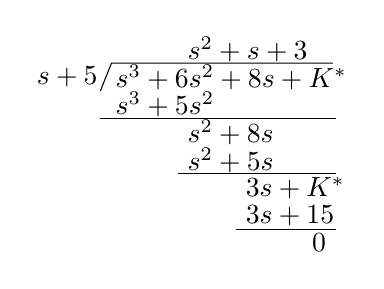
\begin{tikzpicture}[x = 1em, y = 1em]
		\node [anchor=west] at (0,0) {$s^2 + s + 3$};
		\node at (-4,-1) {$s + 5$};
		\path [draw] (-2.8,-1.5) -- ++(.4,1) -- ++(8,0);
		\node [anchor=west] at (-2.6,-1) {$s^3 + 6s^2 + 8s + K^*$};
		\node [anchor=west] at (-2.6,-2) {$s^3 + 5s^2$};
		\path [draw] (-2.8,-2.5) -- ++(8.5,0);
		\node [anchor=west] at (0,-3) {$s^2 + 8s$};
		\node [anchor=west] at (0,-4) {$s^2 + 5s$};
		\path [draw] (0,-4.5) -- ++(5.7,0);
		\node [anchor=west] at (2.1,-5) {$3s + K^*$};
		\node [anchor=west] at (2.1,-6) {$3s + 15$};
		\path [draw] (2.1,-6.5) -- ++(3.6,0);
		\node [anchor=west] at (4.5,-7) {$0$};
	\end{tikzpicture}\\
	$\Rightarrow K^* = 15$，$D(s) = (s + 5)(s^2 + s + 3)$\\
	$\lambda_{1,2} = -0.5 \pm j1.6583$\\
	$K^* = 15$\\
	$K = K^*/8 = 15/8 = 1.875$
\end{frame}

\subsection{开环极点对根轨迹的影响}
\begin{frame}[fragile]{\example{开环极点对根轨迹的影响}{}}
	\emph{系统开环传递函数}
	$(a)~~\frac{K}{s(s+a)}\quad (b)~~\frac{K}{s(s + a)(s + b)} \quad (c)~~\frac{K}{s(s + a)(s + b)(s + c)}$
	\begin{center}
		\begin{tikzpicture}[x=1em,  y=1em]
			\setlayer
			\begin{scope}[xshift=0em]
				\drawaxisnew{-4}{2.5}{-5}{5}{Re}{Im}{a}
				\begin{pgfonlayer}{foreground layer}
					\path[nodes={pole}] (-2,0) node[label=above:$-a$](p1) {} (0,0) node(p2) {};
					\path[nodes={sep}] (-1,0) node(d) {};
				\end{pgfonlayer}
				\path [rlocus] (p1.center) -- (d.center) -- ++(0,4);
				\path [rlocus,blue] (p2.center) -- (d.center) -- ++(0,-4);
			\end{scope}
			\begin{scope}[xshift=11em]
				\drawaxisnew{-6}{2.5}{-5}{5}{Re}{Im}{b}
				\begin{pgfonlayer}{foreground layer}
					\path[nodes={pole}] (-4,0) node[label=above:$-b$](p1) {}(-2,0) node[label=above:$-a$](p2) {} (0,0) node(p3) {};
					\path[nodes={sep}] (-0.845,0) node(d) {};
					\path[nodes={dot}] (0,2.828) node(w1) {} (0,-2.828) node(w2) {};
				\end{pgfonlayer}
				\path [rlocus] (p1.center) -- (-6.5,0);
				\path [rlocus] (p2.center) -- (d.center) .. controls ($(d)+(90:1.5)$) and ($(w1)+(-130:0.5em)$) .. (1.2,5);
				\path [rlocus,blue] (p3.center) -- (d.center) .. controls ($(d)+(-90:1.5)$) and ($(w2)+(130:0.5em)$) .. (1.2,-5);
			\end{scope}
			\begin{scope}[xshift=22em]
				\drawaxisnew{-6}{2.5}{-5}{5}{Re}{Im}{c}
				\begin{pgfonlayer}{foreground layer}
					\path[nodes={pole}] (-6,0) node[label=above:$-c$](p1) {} (-4,0) node[label=above:$-b$](p2) {}(-2,0) node[label=above:$-a$](p3) {} (0,0) node(p4) {};
					\path[nodes={sep}] (-5.155,0) node(d1) {} (-0.845,0) node(d2) {};
					\path[nodes={dot}] (0,2.828) node(w1) {} (0,-2.828) node(w2) {};
					\path (-6,2.828) node(w3) {} (-6,-2.828) node(w4) {};
				\end{pgfonlayer}
				\path [rlocus] (p1.center) -- (d1.center) .. controls ($(d1)+(90:1.5)$) and ($(w3)+(130:0.5em)$) .. (-7.2,5);
				\path [rlocus,blue] (p2.center) -- (d1.center) .. controls ($(d1)+(-90:1.5)$) and ($(w4)+(-130:0.5em)$) .. (-7.2,-5);
				\path [rlocus] (p3.center) -- (d2.center) .. controls ($(d2)+(90:1.5)$) and ($(w1)+(-130:0.5em)$) .. (1.2,5);
				\path [rlocus,blue] (p4.center) -- (d2.center) .. controls ($(d2)+(-90:1.5)$) and ($(w2)+(130:0.5em)$) .. (1.2,-5);
			\end{scope}
		\end{tikzpicture}
	\end{center}
	大致上讲，在开环传递函数加入左半平面的极点具有将原来的根轨迹向右半平面推的效果。
\end{frame}

\subsection{开环零点对根轨迹的影响}
\begin{frame}{\example{开环零点对根轨迹的影响}{}}
	\emph{系统开环传递函数}
	$(a)~~\frac{K}{s(s+a)}\quad (b)~~\frac{K(s + b)}{s(s + a)}$
	\begin{center}
		\begin{tikzpicture}[x=1em,  y=1em]
			\setlayer
			\begin{scope}[xshift=0em]
				\drawaxisnew{-4}{2.5}{-5}{5}{Re}{Im}{a}
				\begin{pgfonlayer}{foreground layer}
					\path[nodes={pole}](-2,0) node[label=above:$-a$](p1) {} (0,0) node(p2) {};
					\path[nodes={sep}] (-1,0) node(d) {};
				\end{pgfonlayer}
				\path [rlocus] (p1.center) -- (d.center) -- ++(0,4);
				\path [rlocus,blue] (p2.center) -- (d.center) -- ++(0,-4);
			\end{scope}
			\begin{scope}[xshift=13em]
				\drawaxisnew{-6}{2.5}{-5}{5}{Re}{Im}{b}
				\begin{pgfonlayer}{foreground layer}
					\path[nodes={pole}](-3,0) node[label=above:$-a$](p1) {} (0,0) node(p2) {};
					\path[nodes={zero}] (-4,0) node[label=below:$-b$](z) {};
					\path[nodes={sep}] (-6.5,0) node(d1) {} (-1.5,0) node(d2) {};
				\end{pgfonlayer}
        			\path [rlocus] (p1.center) -- (d2.center) arc (0:180:2.5) -- +(-2,0);
        			\path [rlocus,blue] (p2.center) -- (d2.center) arc (0:-180:2.5) -- (z);
			\end{scope}
		\end{tikzpicture}
	\end{center}
	大致上讲，在开环传递函数中加入左半平面的零点具有使原来的根轨迹向左半平面推移的效果。
\end{frame}

\addtocounter{example}{-1}
\begin{frame}{\example{[续]开环零点对根轨迹的影响}{}}
	\emph{系统开环传递函数}
	$(c)~~\frac{K}{s(s+a)(s+b)}\quad (d)~~\frac{K(s + c)}{s(s + a)(s+b)}$
	\begin{center}
		\begin{tikzpicture}[x=1em,  y=1em]
			\setlayer
			\begin{scope}[xshift=0em]
				\drawaxisnew{-6}{2.5}{-5}{5}{Re}{Im}{c}
				\begin{pgfonlayer}{foreground layer}
					\path[nodes={pole}](-4,0) node[label=above:$-b$](p1) {}(-2,0) node[label=above:$-a$](p2) {} (0,0) node(p3) {};
					\path[nodes={sep}] (-0.845,0) node(d) {};
					\path[nodes={dot}] (0,2.828) node(w1) {} (0,-2.828) node(w2) {};
				\end{pgfonlayer}
				\path [rlocus] (p1.center) -- (-6.5,0);
				\path [rlocus] (p2.center) -- (d.center) .. controls ($(d)+(90:1.45)$) and ($(w1)+(-130:0.5em)$) .. (1.2,5);
				\path [rlocus,blue] (p3.center) -- (d.center) .. controls ($(d)+(-90:1.45)$) and ($(w2)+(130:0.5em)$) .. (1.2,-5);
			\end{scope}
			\begin{scope}[xshift=12em]
				\drawaxisnew{-6}{2.5}{-5}{5}{Re}{Im}{d}
				\begin{pgfonlayer}{foreground layer}
					\path[nodes={pole}](-4,0) node[label=above:$-b$](p1) {}(-2,0) node[label=above:$-a$](p2) {} (0,0) node(p3) {};
					\path[nodes={zero}] (-6,0) node[label=above:$-c$](z) {};
					\path[nodes={sep}] (-0.845,0) node(d) {};
				\end{pgfonlayer}
				\path [rlocus] (p1.center) -- (z);
				\path [rlocus] (p2.center) -- (d.center) .. controls ($(d)+(90:1em)$) and ($(-.5,2)+(-120:0.5em)$) .. (-.5,5);
				\path [rlocus,blue] (p3.center) -- (d.center) .. controls ($(d)+(-90:1em)$) and ($(-.5,-2)+(120:0.5em)$) .. (-.5,-5);
			\end{scope}
		\end{tikzpicture}
	\end{center}
	大致上讲，在开环传递函数中加入左半平面的零点具有使原来的根轨迹向左半平面推移的效果。
\end{frame}

\subsection{课程小结}
\begin{frame}{课程小结}
	$$\text{绘制根轨迹}\xrightarrow[\text{闭环零极点}]{\text{依条件定}}\left\{\begin{array}{l}
		1~\text{相角条件}\\
		2~\text{模值条件}\\
		3~\text{试根}\\
		4~\text{长除法}\\
		5~\text{根之和}\\
		6~\text{比较系数}\\
		7~\text{解根}
	\end{array}\right.$$
\end{frame}

\end{document}